\section{Langkah-Langkah Percobaan}

Praktikum ini melibatkan serangkaian konfigurasi pada dua perangkat MikroTik RouterBoard, yaitu Router A yang berfungsi sebagai router utama dengan kapabilitas NAT dan Firewall, serta Router B yang dikonfigurasi sebagai perangkat bridge. Pengujian fungsionalitas dilakukan pada perangkat laptop yang terhubung ke infrastruktur jaringan yang dibangun.

\subsection{Konfigurasi Router A (MikroTik)}

\subsubsection*{Reset Konfigurasi Router}
Tahap awal dalam praktikum ini adalah memastikan Router A berada dalam kondisi konfigurasi default guna menghindari potensi konflik pengaturan sebelumnya. Proses ini diawali dengan mengakses router menggunakan aplikasi Winbox. Setelah terhubung, navigasi dilakukan ke menu \texttt{System > Reset Configuration}. Penting untuk mengaktifkan opsi \texttt{"No Default Configuration"} dengan mencentangnya sebelum mengeksekusi perintah \texttt{"Reset Configuration"} untuk memulai proses reset.

\subsubsection*{Akses Router via Winbox}
Setelah proses reset selesai, router dapat diakses kembali melalui aplikasi Winbox. Koneksi dapat dibangun baik melalui MAC address perangkat maupun alamat IP default. Login dilakukan menggunakan username \texttt{"admin"} tanpa kata sandi.

\subsubsection*{Konfigurasi DHCP Client pada Ether 1}
Konektivitas internet Router A diinisiasi dengan menghubungkan kabel internet ke antarmuka \texttt{ether1}. Selanjutnya, konfigurasi DHCP Client dilakukan untuk memperoleh alamat IP secara otomatis dari penyedia layanan internet. Prosedur ini mencakup akses ke menu \texttt{IP > DHCP Client}, penambahan entri baru dengan memilih \texttt{"ether1"} sebagai antarmuka, dan aplikasi konfigurasi. Verifikasi keberhasilan ditandai dengan status koneksi yang menunjukkan \texttt{"bound"}.

\begin{figure}[H]
    \centering
    \begin{minipage}[t]{0.48\textwidth}
        \centering
        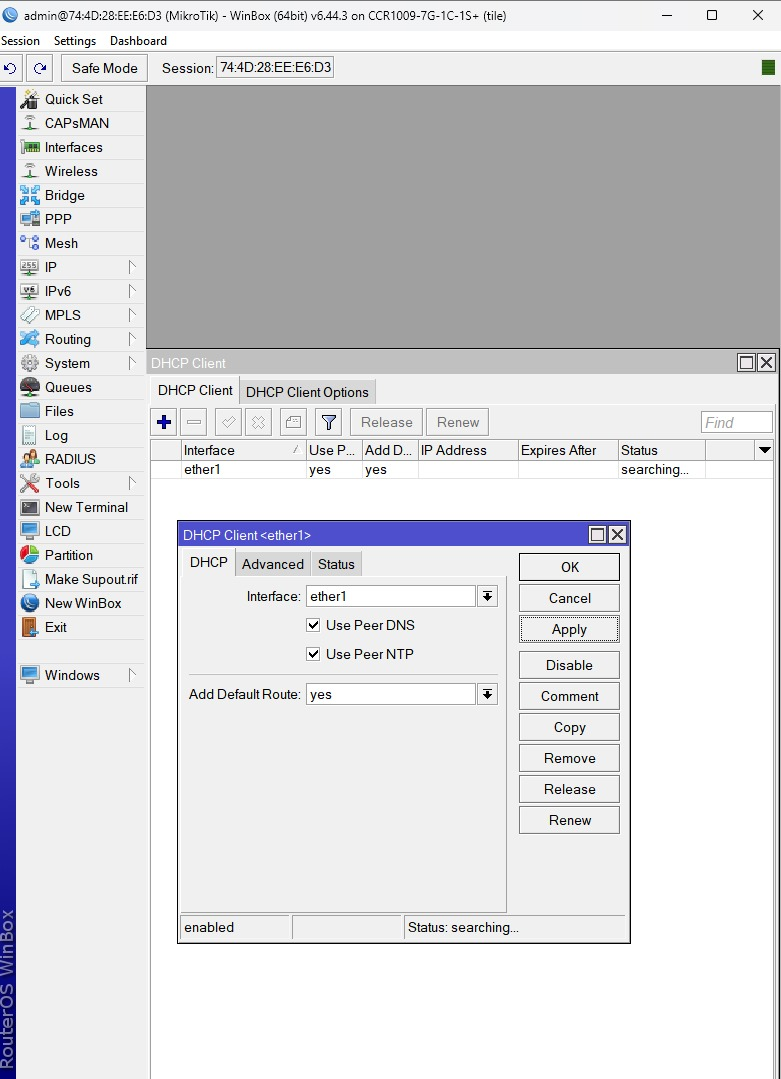
\includegraphics[width=\linewidth]{P1/img/Konfigurasi DHCP Router A.jpg}
        \caption{Konfigurasi DHCP Client pada Ether 1}
        \label{fig:dhcp_client_config}
    \end{minipage}
    \hfill
    \begin{minipage}[t]{0.48\textwidth}
        \centering
        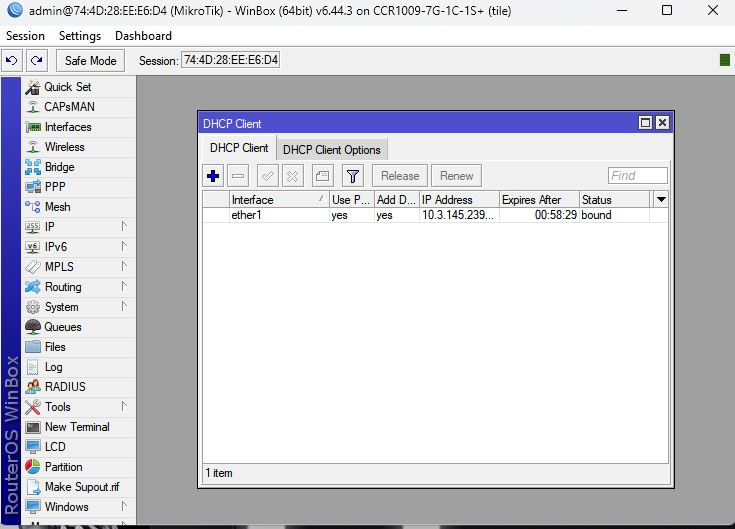
\includegraphics[width=\linewidth]{P1/img/DHCP Bound Router A.jpg}
        \caption{Status DHCP Client "bound" pada Ether 1}
        \label{fig:dhcp_client_bound}
    \end{minipage}
\end{figure}

\subsubsection*{Penambahan Alamat IP pada Ether 7}
Untuk memfasilitasi konektivitas dengan jaringan lokal melalui Switch, alamat IP ditambahkan pada antarmuka \texttt{ether7} Router A. Prosedur ini melibatkan navigasi ke menu \texttt{IP > Addresses}, penambahan alamat IP \texttt{192.168.10.1/24}, dan pemilihan \texttt{"ether7"} sebagai antarmuka. Konfigurasi kemudian diterapkan dan disimpan.

\subsubsection*{Konfigurasi DHCP Server}
Distribusi alamat IP secara otomatis kepada perangkat klien di jaringan lokal dilakukan melalui konfigurasi DHCP Server pada Router A. Proses ini diawali dengan akses ke menu \texttt{IP > DHCP Server} dan penggunaan fitur \texttt{"DHCP Setup"}. Langkah-langkah selanjutnya meliputi pemilihan \texttt{"ether7"} sebagai antarmuka DHCP Server, verifikasi ruang alamat DHCP (\texttt{192.168.10.0/24}), penetapan gateway (\texttt{192.168.10.1}), penentuan rentang IP yang akan didistribusikan (\texttt{192.168.10.2-192.168.10.254}), serta konfigurasi DNS Server (\texttt{8.8.8.8} dan \texttt{8.8.4.4}) dan waktu lease (\texttt{00:10:00}). Konfigurasi berhasil apabila muncul pesan \texttt{"Setup has completed successfully"}.

\begin{figure}[H]
    \centering
    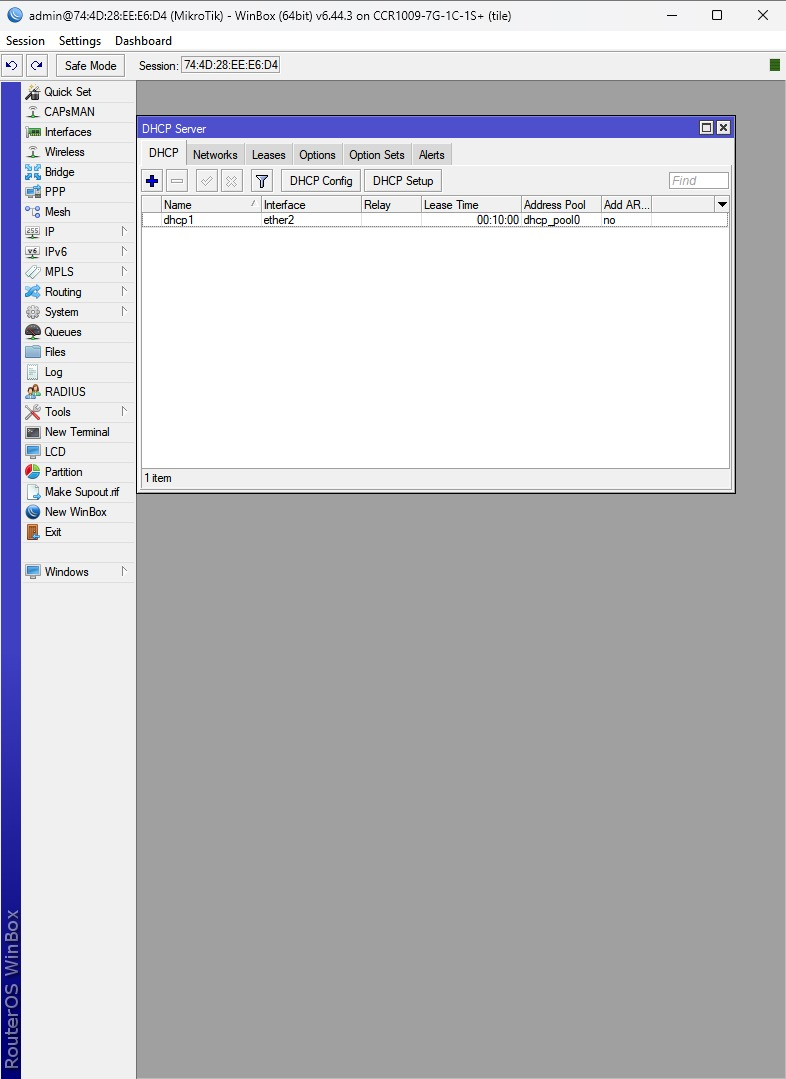
\includegraphics[width=0.7\textwidth]{P1/img/DHCP Server Router A.jpg} %
    \caption{Tampilan Konfigurasi DHCP Server pada Router A}
    \label{fig:dhcp_server_router_a}
\end{figure}

\subsubsection*{Konfigurasi NAT}
NAT (Network Address Translation) dikonfigurasi untuk memungkinkan perangkat di jaringan lokal mengakses internet. Konfigurasi ini dilakukan melalui menu \texttt{IP > Firewall > NAT}. Aturan baru ditambahkan dengan Chain \texttt{"src-nat"} pada tab \texttt{"General"}, dan Action \texttt{"masquerade"} pada tab \texttt{"Action"}. Implementasi NAT ini esensial untuk penerjemahan alamat IP privat ke alamat IP publik.

\begin{figure}[H]
    \centering
    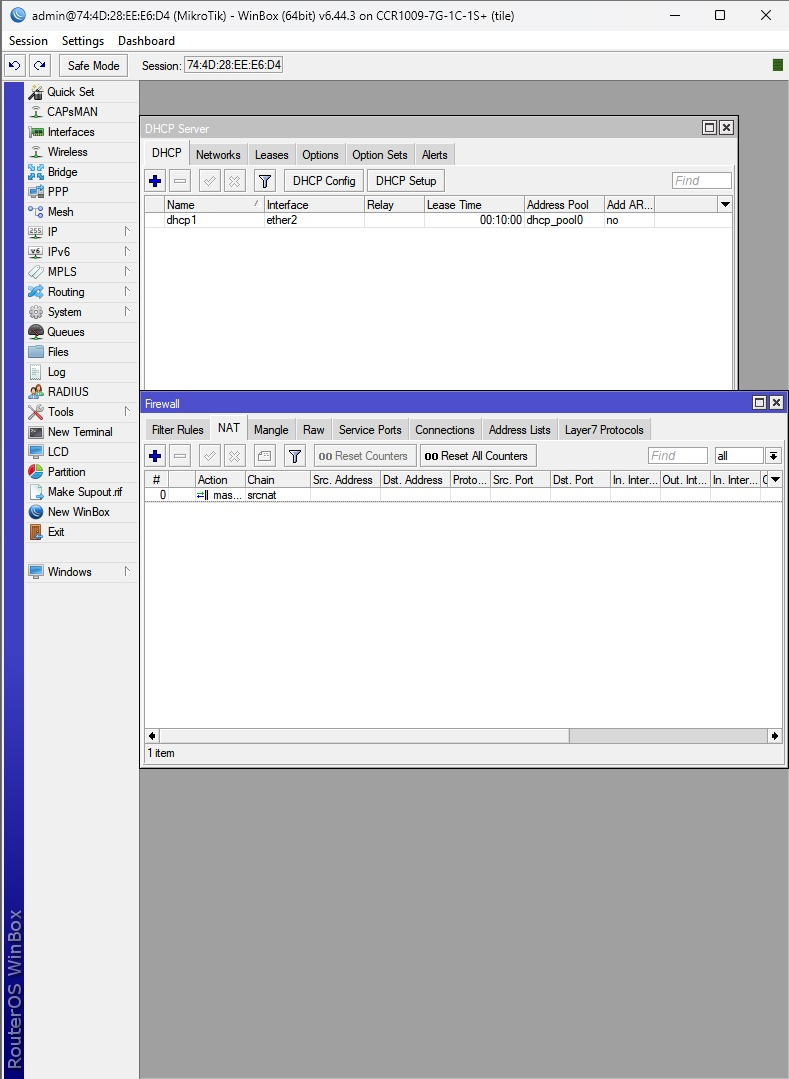
\includegraphics[width=0.7\textwidth]{P1/img/Konfigurasi NAT.jpg} %
    \caption{Tampilan Konfigurasi NAT pada Router A}
    \label{fig:konfigurasi_nat}
\end{figure}

\subsubsection*{Konfigurasi Firewall (Filter Rules)}
Penerapan aturan filter (Filter Rules) pada firewall bertujuan untuk mengatur lalu lintas jaringan dan meningkatkan keamanan. Ini diatur melalui menu \texttt{IP > Firewall > Filter Rule}.

Untuk pemblokiran ICMP (Internet Control Message Protocol), aturan baru ditambahkan dengan Chain \texttt{"forward"}, Protocol \texttt{"icmp"}, dan In. Interface \texttt{"ether7"} pada tab \texttt{"General"}. Pada tab \texttt{"Action"}, Action diatur menjadi \texttt{"drop"}. Konfigurasi ini dirancang untuk memblokir permintaan ping yang masuk dari jaringan lokal ke luar.

\begin{figure}[H]
    \centering
    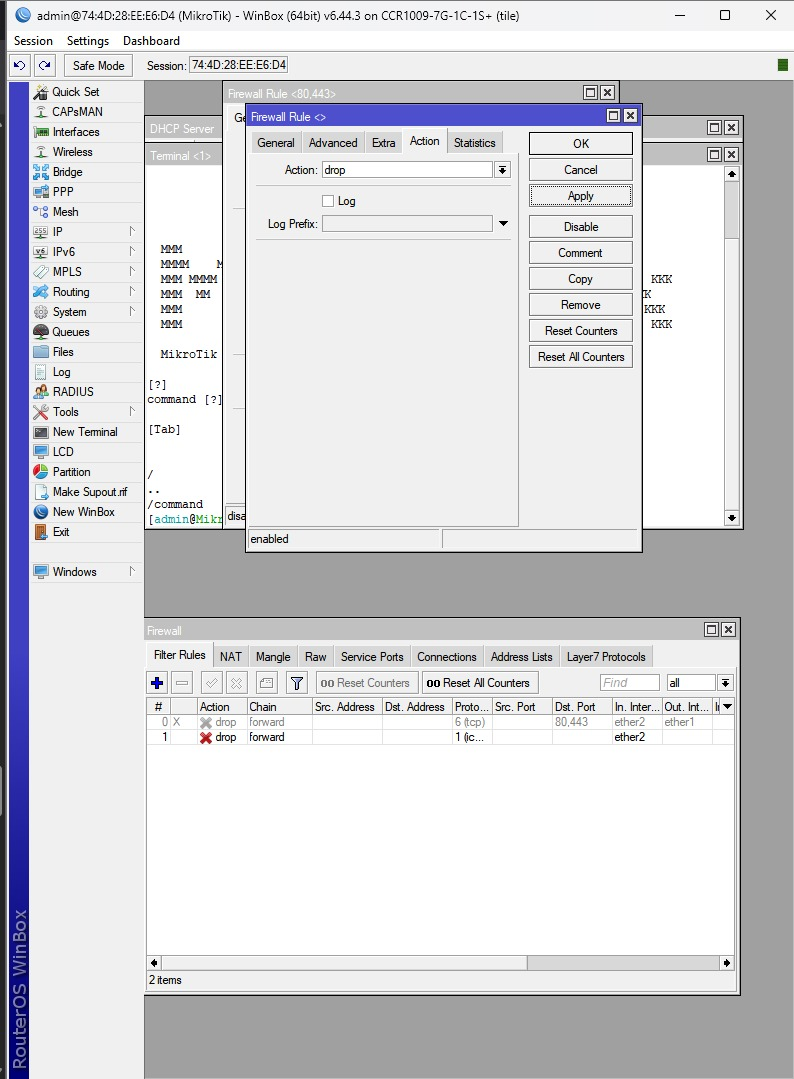
\includegraphics[width=0.7\textwidth]{P1/img/ICMP Block.jpg} %
    \caption{Tampilan Konfigurasi Firewall untuk Pemblokiran ICMP}
    \label{fig:icmp_block_config}
\end{figure}

Selanjutnya, untuk pemblokiran akses situs web berdasarkan konten spesifik (misalnya, "speedtest"), aturan firewall lainnya ditambahkan. Aturan ini memiliki Chain \texttt{"forward"}, Protocol \texttt{"tcp"}, dan Dst. Port \texttt{"80,443"} pada tab \texttt{"General"}. In. Interface diatur ke \texttt{"ether7"} dan Out. Interface ke \texttt{"ether1"}. Pada tab \texttt{"Advanced"}, Content diatur ke \texttt{"speedtest"}, dan Action diatur menjadi \texttt{"drop"}. Aturan ini berfungsi untuk memblokir akses ke situs web yang mengandung kata kunci "speedtest" dalam lalu lintas HTTP/HTTPS.

\begin{figure}[H]
    \centering
    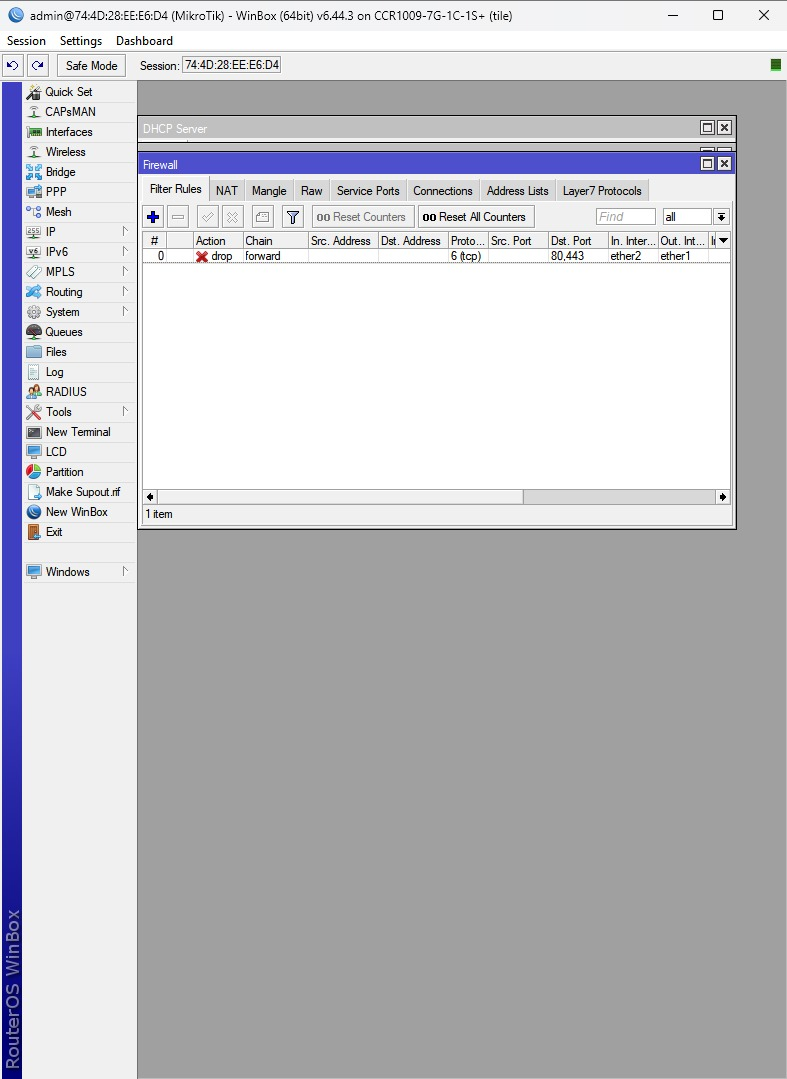
\includegraphics[width=0.7\textwidth]{P1/img/Content Blocking.jpg} %
    \caption{Tampilan Konfigurasi Firewall untuk Pemblokiran Konten "speedtest"}
    \label{fig:content_blocking_config}
\end{figure}

\subsection{Konfigurasi Bridge pada Router B}
Router B dikonfigurasi sebagai perangkat bridge untuk berfungsi sebagai hub yang mentransmisikan lalu lintas antar antarmuka tanpa melakukan routing. Konfigurasi ini diawali dengan mengakses menu \texttt{Bridge} dan membuat bridge baru. Setelah bridge berhasil dibuat, port-port yang terhubung ke perangkat laptop dan Router A ditambahkan ke dalam bridge melalui menu \texttt{Bridge > Port}.

\begin{figure}[H]
    \centering
    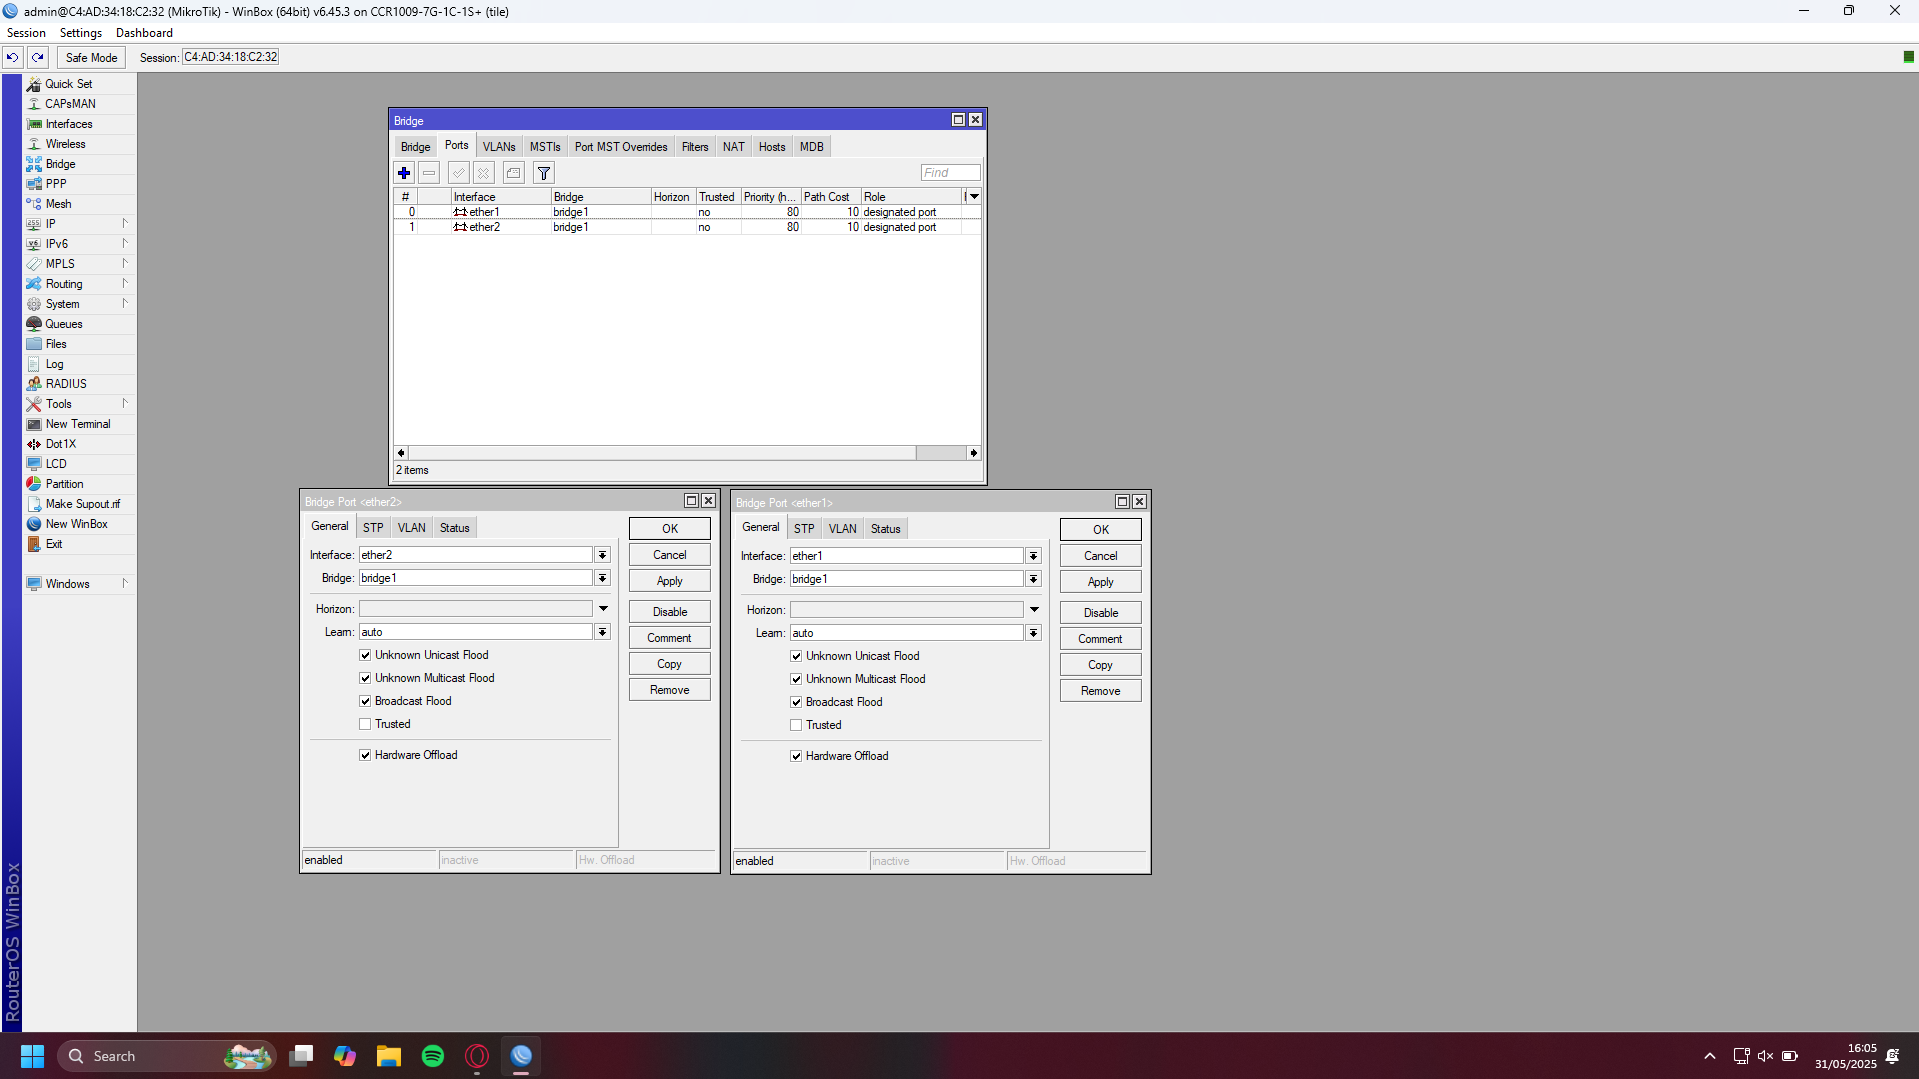
\includegraphics[width=0.7\textwidth]{P1/img/Konfigurasi Bridge.png} %
    \caption{Tampilan Konfigurasi Bridge pada Router B}
    \label{fig:bridge_config}
\end{figure}

\subsection{Konfigurasi Alamat IP pada Laptop}
Sebagai bagian dari pengujian, konfigurasi alamat IP pada laptop diatur untuk memperoleh alamat secara otomatis melalui DHCP. Verifikasi perolehan alamat IP dilakukan dengan membuka Command Prompt (CMD) dan mengeksekusi perintah \texttt{ipconfig}.

\section{Analisis Hasil Percobaan}

Pengujian fungsionalitas NAT dan Firewall dilakukan setelah seluruh konfigurasi perangkat selesai. Analisis ini membahas hasil dari setiap pengujian yang dilakukan.

\subsection{Pengujian Konektivitas (NAT)}
Pengujian konektivitas internet dilakukan untuk memverifikasi fungsi NAT setelah konfigurasi DHCP Client, IP Addresses, DHCP Server, dan NAT pada Router A. Dengan mengeksekusi perintah \texttt{ping 8.8.8.8} dari Terminal Winbox, diperoleh balasan (\texttt{reply}) dari \texttt{8.8.8.8}. Hasil ini mengindikasikan bahwa Router A berhasil memperoleh koneksi internet dari penyedia layanan dan fungsi NAT berjalan dengan baik, memungkinkan penerjemahan alamat IP privat dari jaringan lokal ke alamat IP publik untuk akses internet.

\subsection{Pengujian Firewall (ICMP)}
Pengujian terhadap aturan pemblokiran ICMP (ping) dilakukan dari perangkat laptop ke internet. Tabel di bawah merangkum hasil pengujian:

\begin{longtable}{|p{0.2\textwidth}|p{0.3\textwidth}|p{0.4\textwidth}|}
\caption{Hasil Pengujian Firewall ICMP} \label{tab:icmp_test} \\
\hline
\textbf{Kondisi Firewall} & \textbf{Tindakan/Perintah} & \textbf{Hasil} \\
\hline
\endfirsthead
\multicolumn{3}{c}%
{\tablename\ \thetable\ -- Lanjutan dari halaman sebelumnya} \\
\hline
\textbf{Kondisi Firewall} & \textbf{Tindakan/Perintah} & \textbf{Hasil} \\
\hline
\endhead
\hline
\endfoot
\hline
\endlastfoot
Firewall ICMP Aktif & \texttt{ping 8.8.8.8} dari Laptop & \texttt{Request Timed Out (RTO)} \\
\hline
Firewall ICMP Nonaktif & Aturan firewall ICMP di-disable & Mendapatkan balasan (\texttt{reply}) \\
\hline
\end{longtable}

Berdasarkan hasil tersebut, dapat disimpulkan bahwa aturan firewall untuk ICMP berfungsi secara efektif. Ketika aturan aktif, lalu lintas ping berhasil diblokir, menghasilkan \texttt{Request Timed Out}. Sebaliknya, ketika aturan dinonaktifkan, lalu lintas ping diizinkan dan menghasilkan balasan normal. Hal ini memvalidasi kemampuan firewall dalam mengontrol lalu lintas ICMP.

\subsection{Pengujian Firewall (Pemblokiran Konten)}
Pengujian selanjutnya adalah verifikasi aturan pemblokiran situs web berdasarkan konten, khususnya kata kunci "speedtest". Tabel berikut menampilkan hasil pengujian:

\begin{longtable}{|p{0.2\textwidth}|p{0.3\textwidth}|p{0.4\textwidth}|}
\caption{Hasil Pengujian Firewall Konten} \label{tab:content_test} \\
\hline
\textbf{Kondisi Firewall} & \textbf{Tindakan/Perintah} & \textbf{Hasil} \\
\hline
\endfirsthead
\multicolumn{3}{c}%
{\tablename\ \thetable\ -- Lanjutan dari halaman sebelumnya} \\
\hline
\textbf{Kondisi Firewall} & \textbf{Tindakan/Perintah} & \textbf{Hasil} \\
\hline
\endhead
\hline
\endfoot
\hline
\endlastfoot
Firewall Konten Aktif & Akses \texttt{www.speedtest.net} dari Laptop & Situs web tidak dapat diakses atau terus memuat tanpa menampilkan konten. \\
\hline
Firewall Konten Nonaktif & Aturan firewall konten di-disable & Situs web dapat diakses dengan normal, menampilkan hasil speedtest. \\
\hline
\end{longtable}

\begin{figure}[H]
    \centering
    \begin{minipage}[t]{0.48\textwidth}
        \centering  
        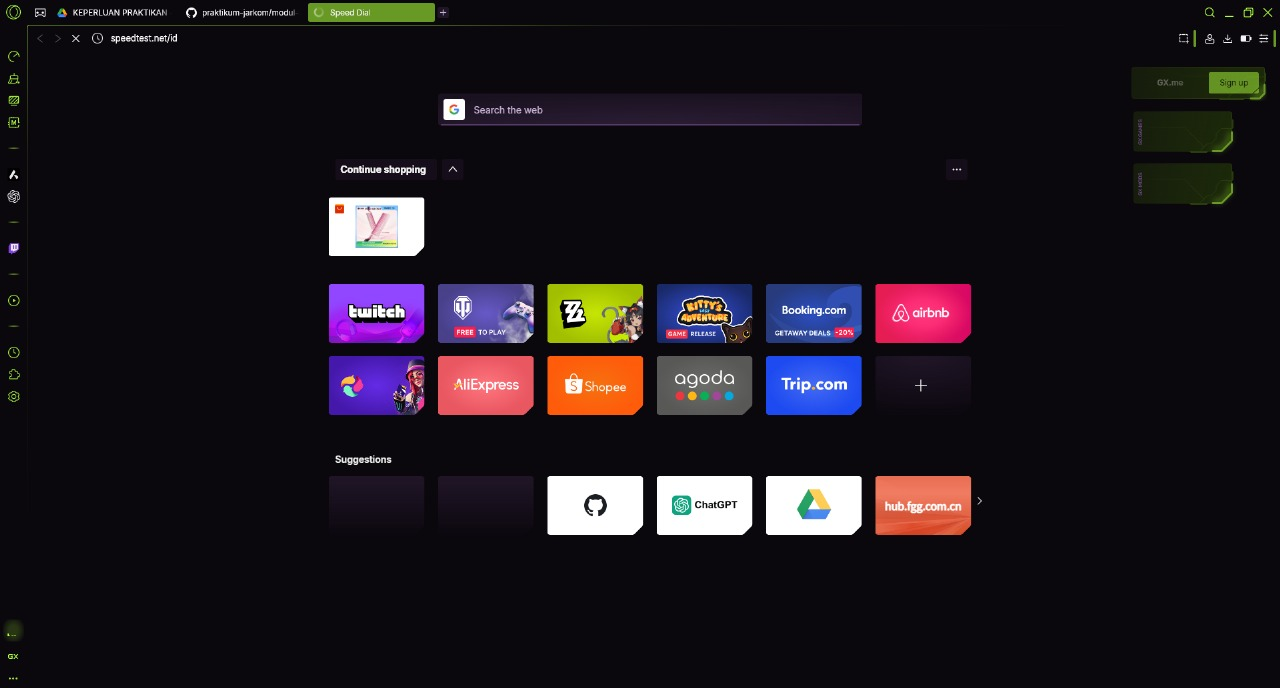
\includegraphics[width=\linewidth]{P1/img/PC2 Ketika Enable Speedtest Block.jpg}
        \caption{Firewall konten aktif}
        \label{fig:ping_acl2_pc0}
    \end{minipage}
    \hfill
    \begin{minipage}[t]{0.48\textwidth}
        \centering
        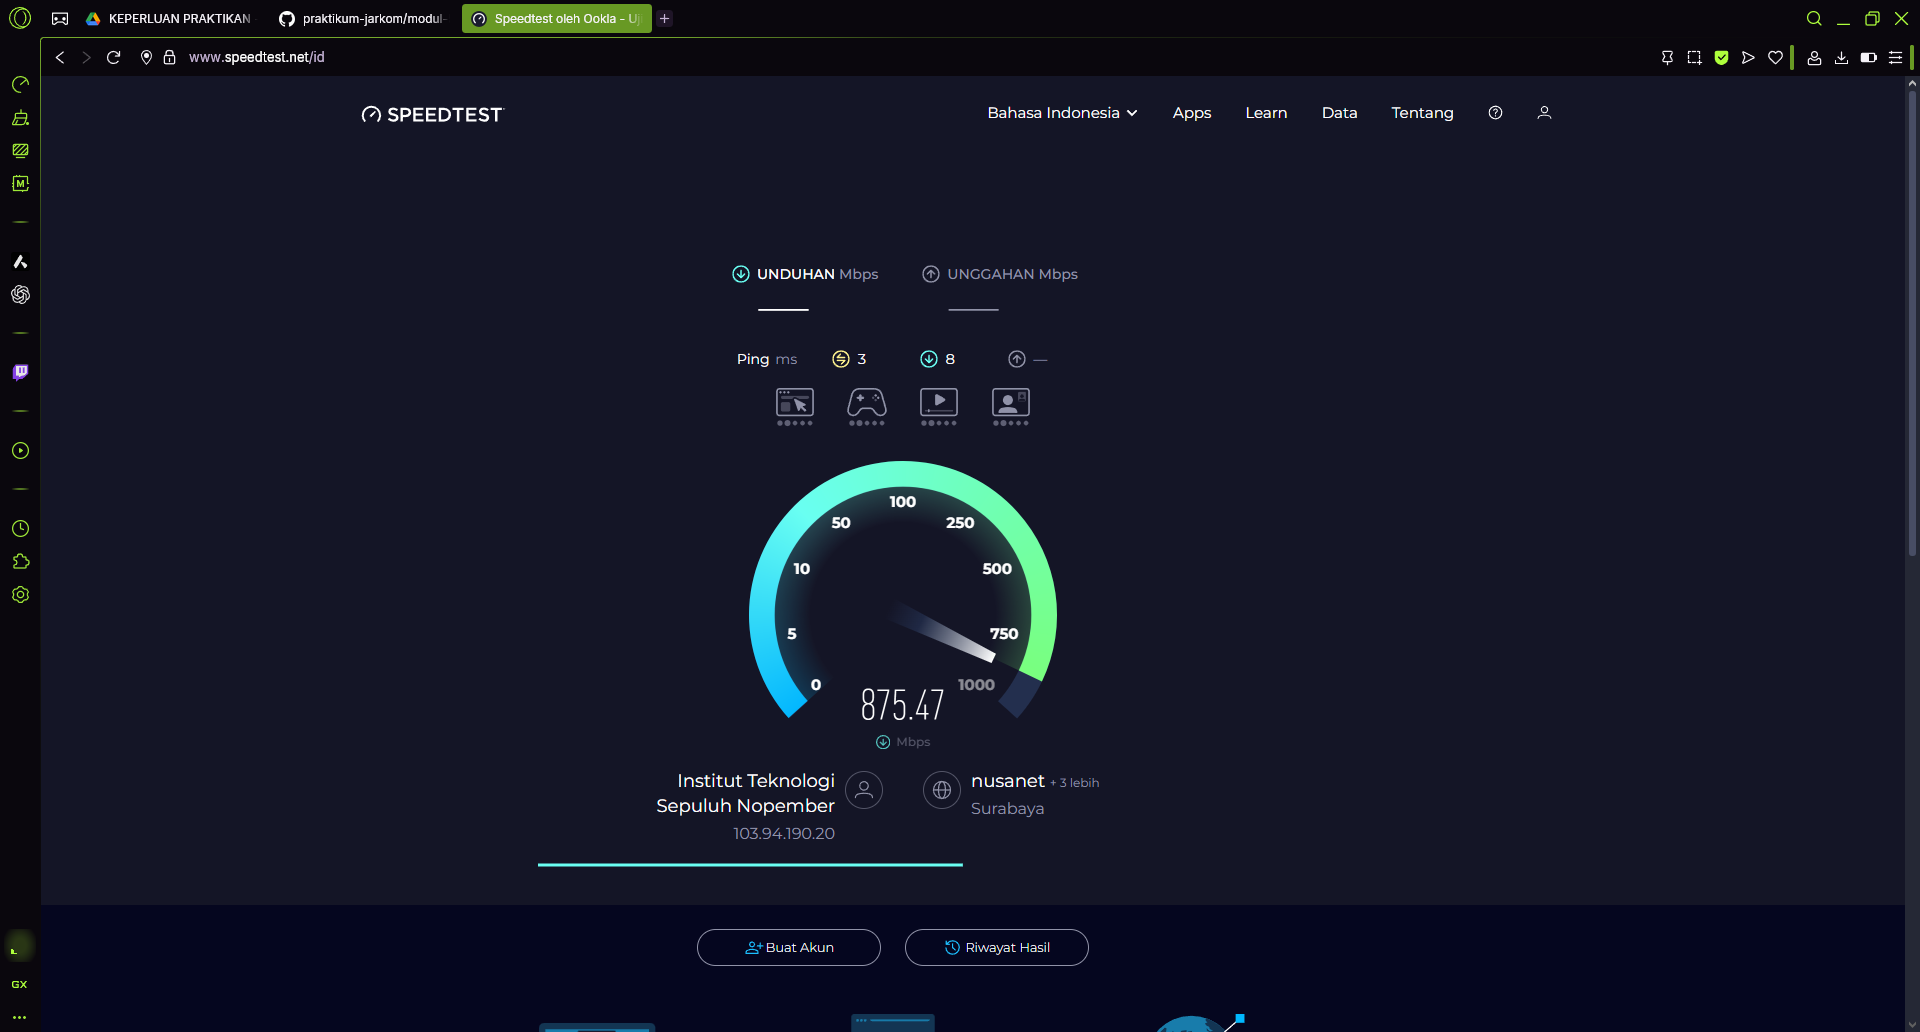
\includegraphics[width=\linewidth]{P1/img/PC2 Ketika Disable Speedtest Block.png}
        \caption{Firewall ketika konten nonaktif}
        \label{fig:ping_acl2_pc1}
    \end{minipage}
\end{figure}

Hasil pengujian ini mengkonfirmasi bahwa firewall konten berhasil memblokir akses ke situs web yang mengandung kata kunci "speedtest" saat aturan diaktifkan, dan mengizinkan akses normal ketika aturan dinonaktifkan. Ini menunjukkan efektivitas firewall dalam melakukan penyaringan konten berbasis kata kunci.

\section{Hasil Tugas Modul}

Tugas ini meliputi pembangunan topologi jaringan sederhana, konfigurasi NAT (Network Address Translation), dan implementasi firewall menggunakan Access Control Lists (ACLs) di Cisco Packet Tracer. Pengujian konektivitas dilakukan untuk memvalidasi setiap konfigurasi.

\subsection*{Topologi Jaringan}
Topologi yang dibangun terdiri dari satu Router (\texttt{2911}), satu Switch (\texttt{2960}), tiga PC (\texttt{PC0}, \texttt{PC1}, \texttt{PC2}) yang terhubung dalam satu jaringan LAN, dan satu Server (\texttt{Server0}) yang disimulasikan sebagai internet/jaringan publik.

\begin{itemize}
    \item \textbf{Router Interface Gig0/0 (LAN)}: \texttt{192.168.1.1/24}
    \item \textbf{Router Interface Gig0/1 (Public)}: \texttt{200.10.10.1/24}
    \item \textbf{PC0 IP}: \texttt{192.168.1.10/24}, Gateway: \texttt{192.168.1.1}
    \item \textbf{PC1 IP}: \texttt{192.168.1.11/24}, Gateway: \texttt{192.168.1.1}
    \item \textbf{PC2 IP}: \texttt{192.168.1.12/24}, Gateway: \texttt{192.168.1.1}
    \item \textbf{Server0 IP}: \texttt{200.10.10.2/24}, Gateway: \texttt{200.10.10.1}
\end{itemize}

 \begin{figure}[H]
     \centering
    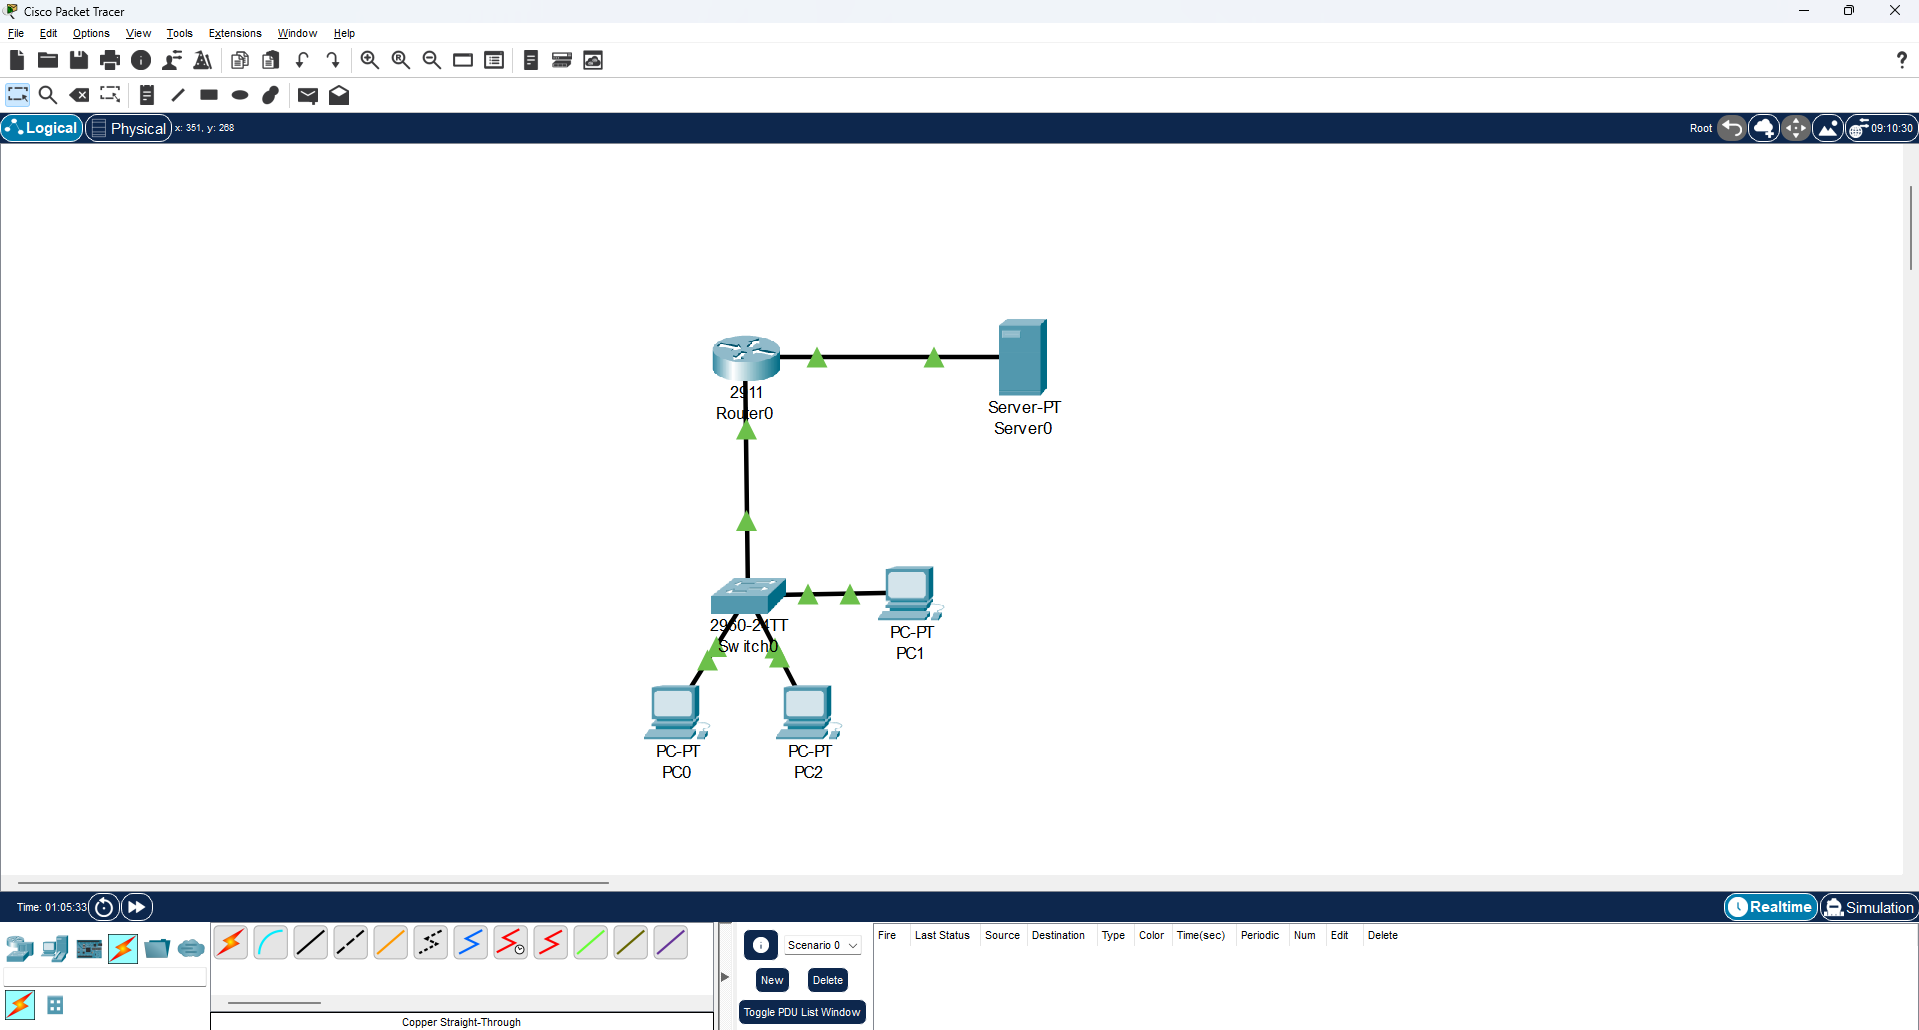
\includegraphics[width=0.8\textwidth]{P1/img/Topologi (2).png} % Ganti dengan nama file gambar Anda
    \caption{Diagram Topologi Jaringan}
     \label{fig:topologi}
 \end{figure}

\subsection*{Konfigurasi NAT (Network Address Translation)}
NAT dikonfigurasi untuk memungkinkan semua PC di jaringan LAN (IP private \texttt{192.168.1.x}) mengakses Server (\texttt{200.10.10.2}) menggunakan IP publik Router (\texttt{200.10.10.1}). Konfigurasi menggunakan NAT Overload (PAT) diterapkan pada Router.

\begin{itemize}
    \item \texttt{access-list 1 permit 192.168.1.0 0.0.0.255}
    \item \texttt{ip nat inside source list 1 interface GigabitEthernet0/1 overload}
    \item \texttt{interface GigabitEthernet0/0}: \texttt{ip nat inside}
    \item \texttt{interface GigabitEthernet0/1}: \texttt{ip nat outside}
\end{itemize}

\textbf{Hasil Pengujian Konektivitas Setelah NAT:}
\begin{itemize}
    \item \texttt{PC0} $\rightarrow$ \texttt{ping 200.10.10.2}: \textbf{Berhasil}
    \item \texttt{PC1} $\rightarrow$ \texttt{ping 200.10.10.2}: \textbf{Berhasil}
    \item \texttt{PC2} $\rightarrow$ \texttt{ping 200.10.10.2}: \textbf{Berhasil}
\end{itemize}
Semua PC di LAN berhasil mengakses Server, memverifikasi fungsi NAT.

\begin{figure}[H]
    \centering
    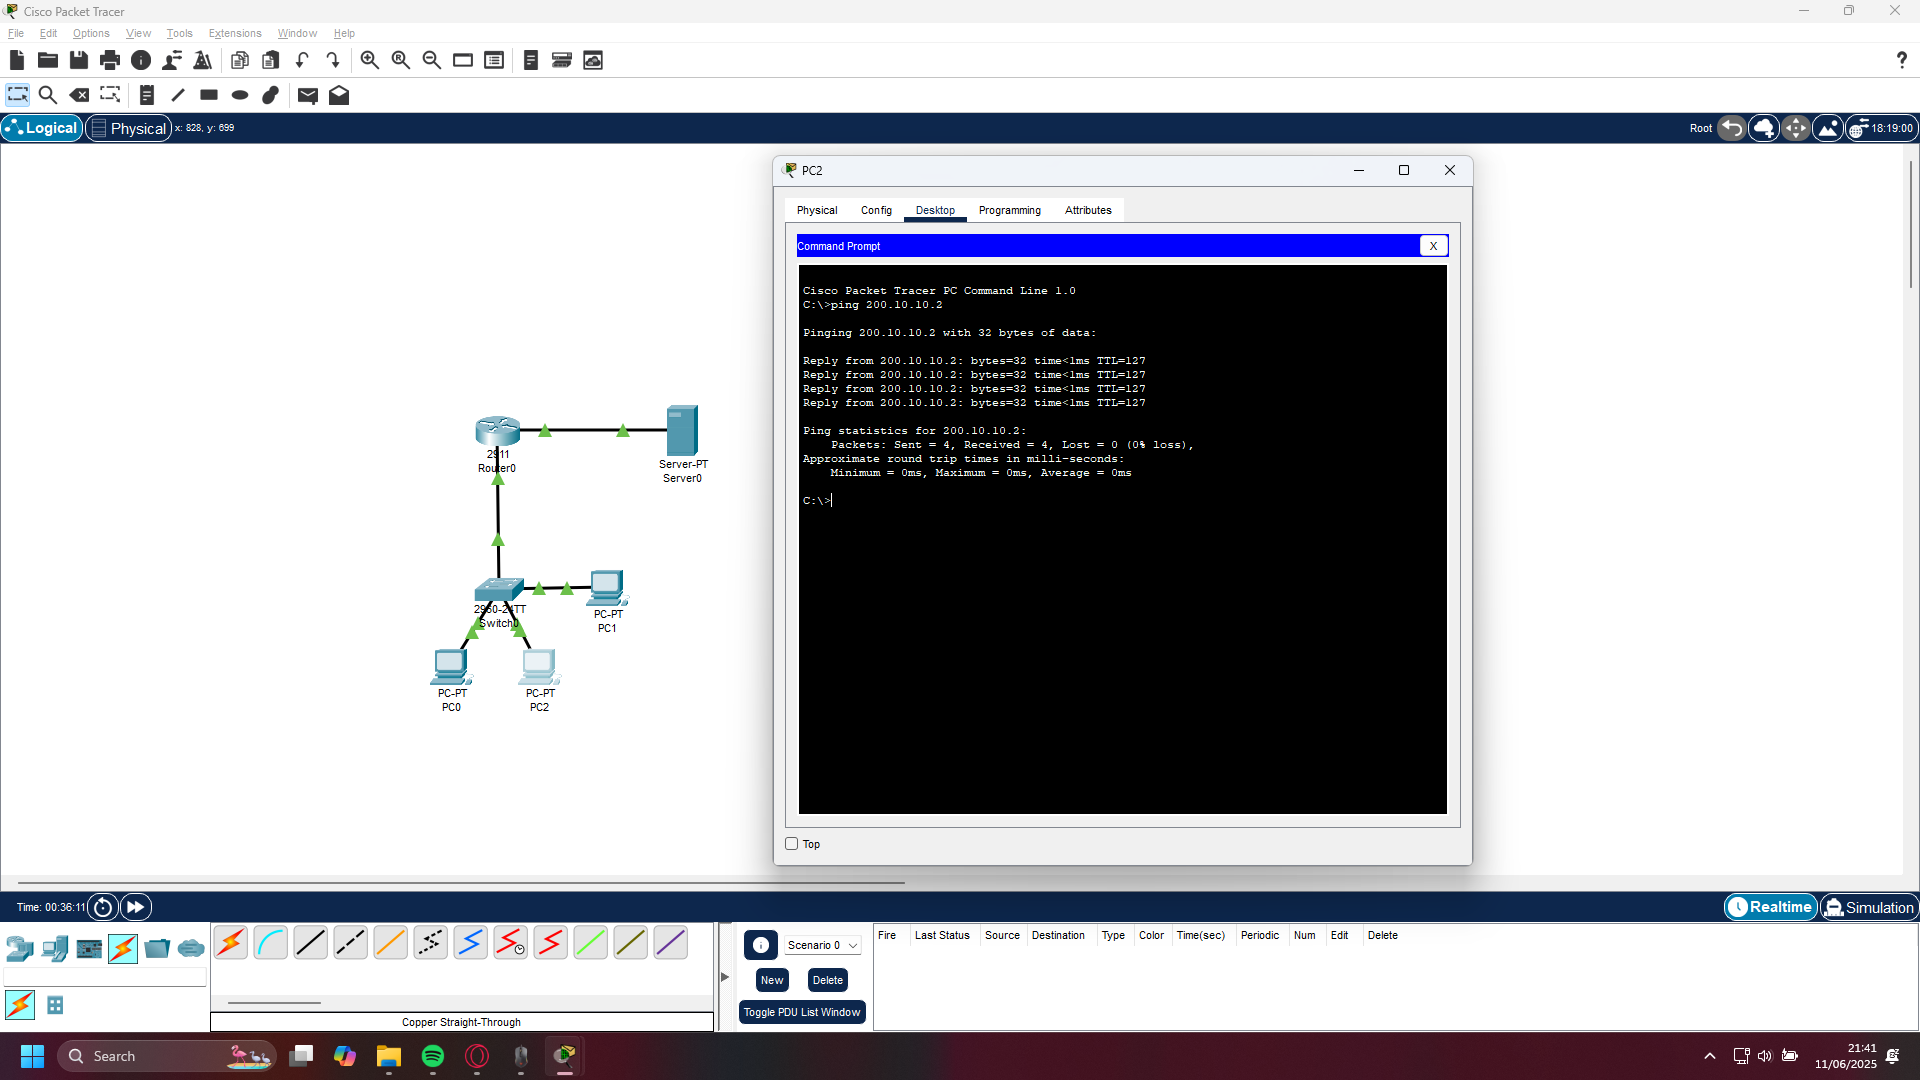
\includegraphics[width=0.7\textwidth]{P1/img/Test Ping Setelah NAT.png} %
    \caption{Hasil Ping ke Server Setelah Konfigurasi NAT (Contoh dari PC2)}
    \label{fig:ping_after_nat}
\end{figure}

\subsection*{Konfigurasi Firewall (ACL)}

Dua skenario ACL diimplementasikan dan diuji untuk mengontrol akses PC ke Server. ACL diterapkan pada \texttt{interface GigabitEthernet0/0} dengan arah \texttt{in} (masuk dari LAN ke router) untuk mengontrol lalu lintas yang keluar dari LAN.

\subsubsection*{Skenario 1: Izinkan Hanya PC1 Mengakses Server}
Dalam skenario ini, ACL dikonfigurasi untuk secara eksplisit mengizinkan hanya \texttt{PC1} (\texttt{192.168.1.11}) untuk mengakses \texttt{Server0} (\texttt{200.10.10.2}). Aturan \texttt{deny any} implisit pada ACL akan memblokir PC lainnya. Untuk skenario ini, NAT static digunakan untuk \texttt{PC1} agar tetap bisa berkomunikasi setelah ACL diaktifkan.

\begin{itemize}
    \item \texttt{ip nat inside source static 192.168.1.11 200.10.10.1}
    \item \texttt{access-list 100 permit ip host 192.168.1.11 host 200.10.10.2}
    \item \texttt{access-list 100 deny ip any host 200.10.10.2}
    \item \texttt{interface GigabitEthernet0/0}: \texttt{ip access-group 100 in}
\end{itemize}

\textbf{Hasil Pengujian Konektivitas Skenario 1:}
\begin{itemize}
    \item \texttt{PC1} $\rightarrow$ \texttt{ping 200.10.10.2}: \textbf{Berhasil}
    \item \texttt{PC0} $\rightarrow$ \texttt{ping 200.10.10.2}: \textbf{Gagal} (Request timed out)
    \item \texttt{PC2} $\rightarrow$ \texttt{ping 200.10.10.2}: \textbf{Gagal} (Request timed out)
    \item \texttt{PCx} $\rightarrow$ \texttt{ping 192.168.1.x} (antar PC LAN): \textbf{Berhasil} (Komunikasi LAN tidak terpengaruh)
\end{itemize}
Pengujian ini menunjukkan bahwa hanya \texttt{PC1} yang diizinkan mengakses Server, sesuai dengan konfigurasi ACL.

\begin{figure}[H]
    \centering
    \begin{minipage}[t]{0.48\textwidth}
        \centering
        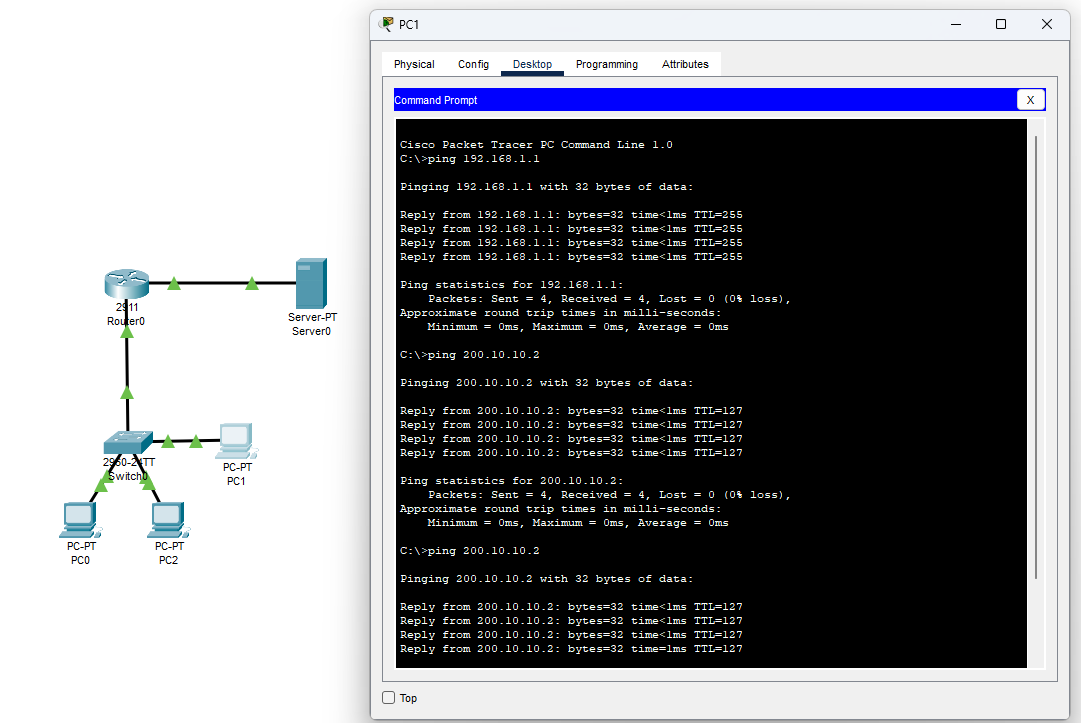
\includegraphics[width=\linewidth]{P1/img/Test Ping ACL Skenario PC1.png}
        \caption{Hasil Ping dari PC1 ke Server (Skenario 1)}
        \label{fig:ping_acl1_pc1}
    \end{minipage}
    \hfill
    \begin{minipage}[t]{0.48\textwidth}
        \centering
        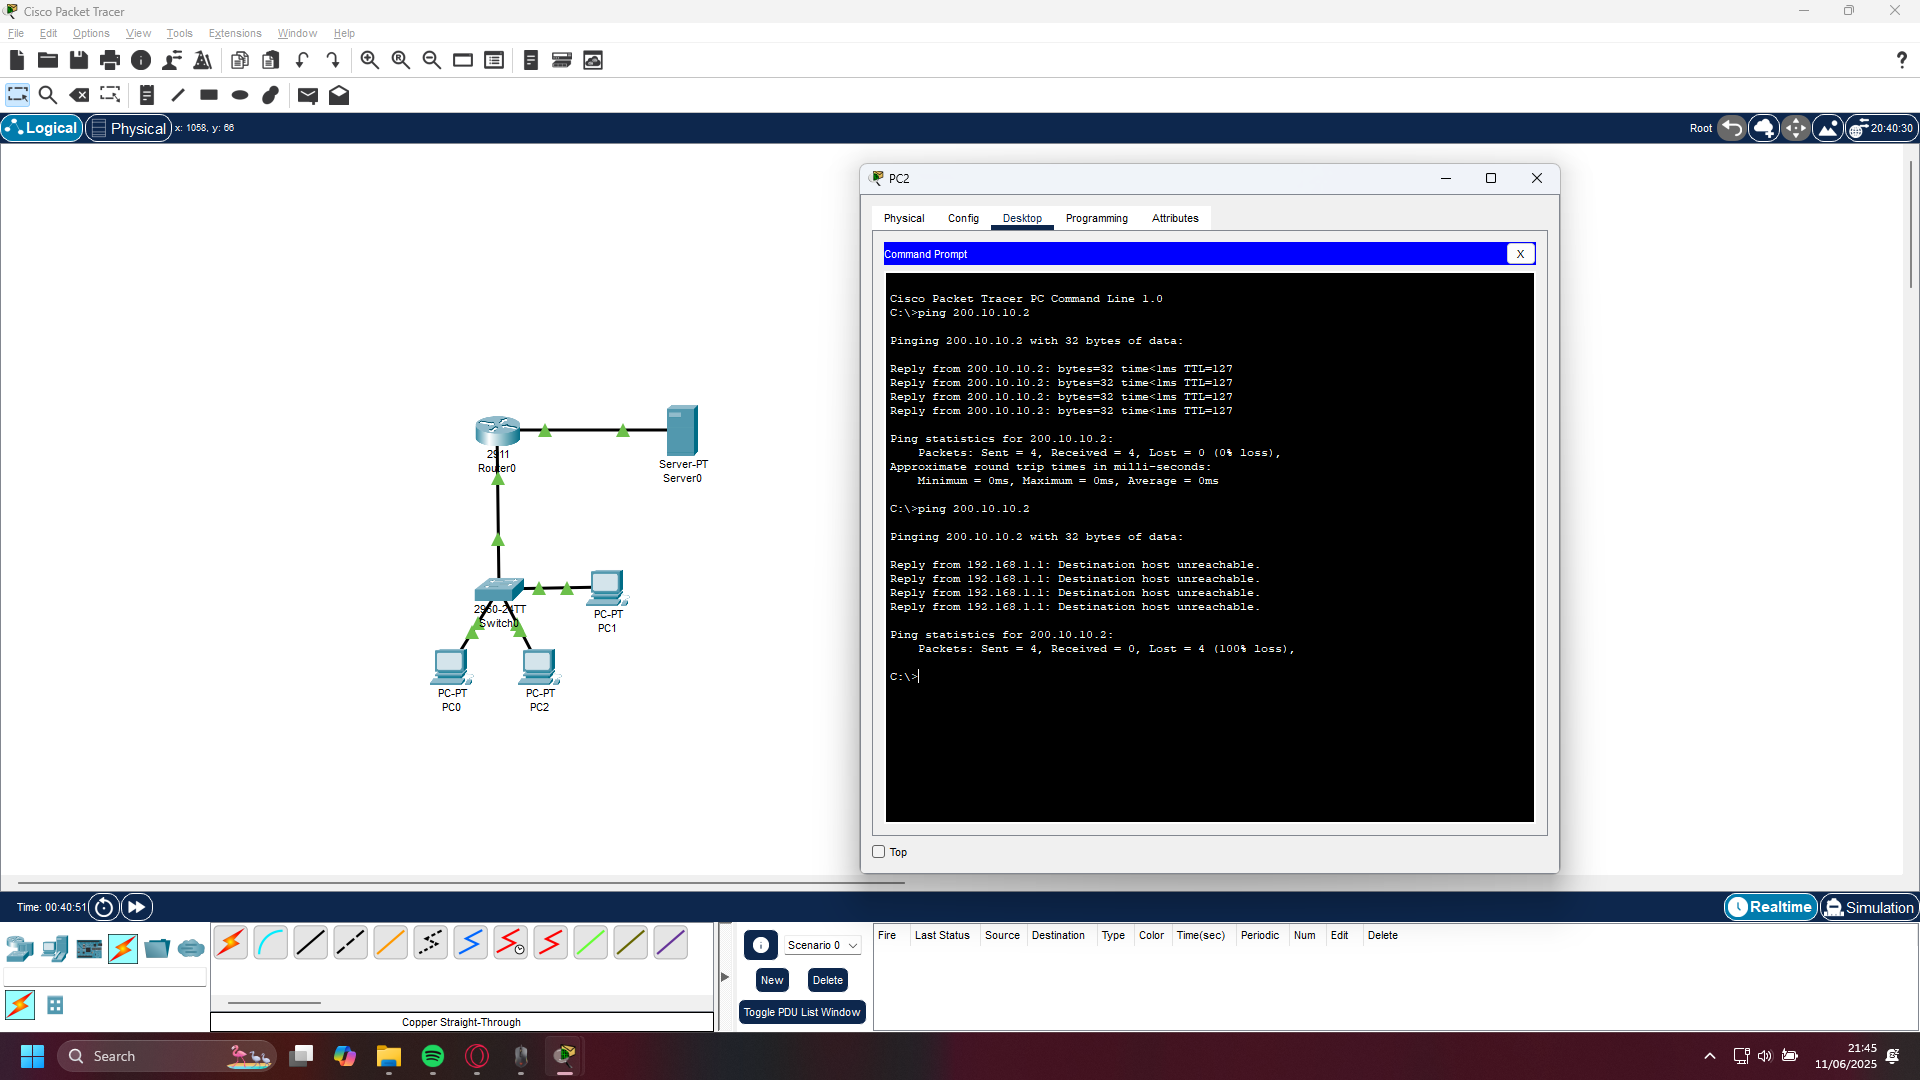
\includegraphics[width=\linewidth]{P1/img/Test Ping ACL Skenario 1 PC2.png}
        \caption{Hasil Ping dari PC2 ke Server (Skenario 1 - Gagal)}
        \label{fig:ping_acl1_pc2}
    \end{minipage}
\end{figure}

\begin{figure}[H]
    \centering
    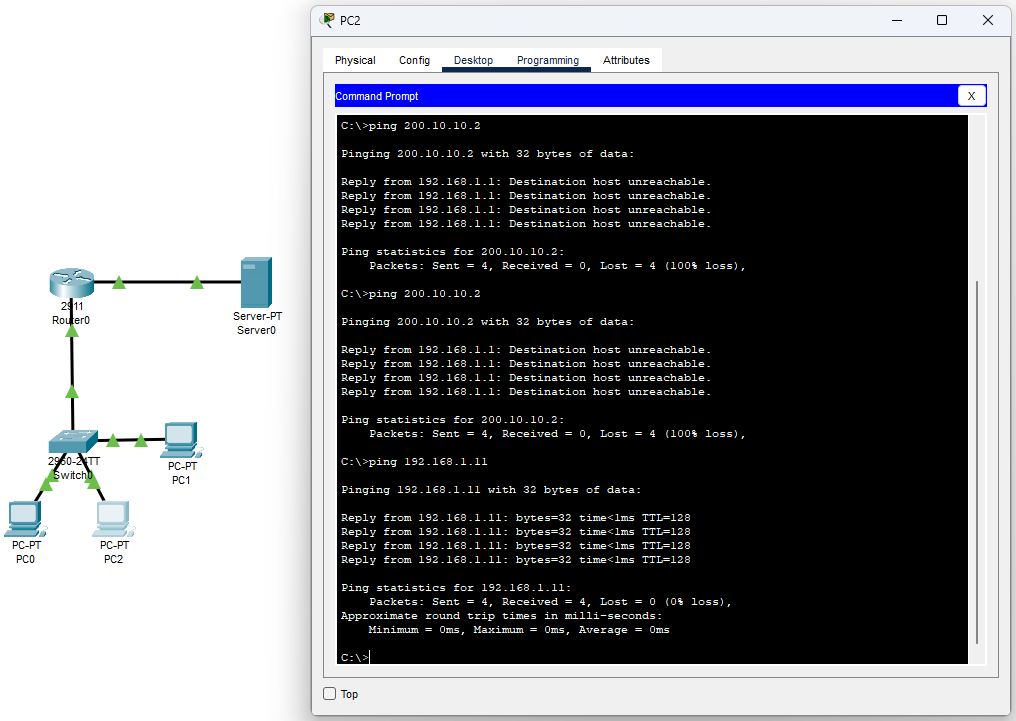
\includegraphics[width=0.48\textwidth]{P1/img/Ping Antar PC di LAN.png}
    \caption{Hasil Ping Antar PC di LAN (Tidak Terpengaruh ACL)}
    \label{fig:ping_lan}
\end{figure}

\subsubsection*{Skenario 2: Blokir PC1 dan PC2 Mengakses Server}
Pada skenario ini, ACL dikonfigurasi untuk secara eksplisit memblokir \texttt{PC1} (\texttt{192.168.1.11}) dan \texttt{PC2} (\texttt{192.168.1.12}) dari mengakses \texttt{Server0}. Aturan \texttt{permit ip any any} ditambahkan di akhir ACL untuk memastikan PC lainnya (\texttt{PC0}) tetap dapat mengakses Server. NAT overload untuk seluruh LAN diaktifkan kembali.

\begin{itemize}
    \item \texttt{access-list 101 deny ip host 192.168.1.11 host 200.10.10.2}
    \item \texttt{access-list 101 deny ip host 192.168.1.12 host 200.10.10.2}
    \item \texttt{access-list 101 permit ip any any}
    \item \texttt{interface GigabitEthernet0/0}: \texttt{ip access-group 101 in}
\end{itemize}

\textbf{Hasil Pengujian Konektivitas Skenario 2:}
\begin{itemize}
    \item \texttt{PC0} $\rightarrow$ \texttt{ping 200.10.10.2}: \textbf{Berhasil}
    \item \texttt{PC1} $\rightarrow$ \texttt{ping 200.10.10.2}: \textbf{Gagal} (Request timed out)
    \item \texttt{PC2} $\rightarrow$ \texttt{ping 200.10.10.2}: \textbf{Gagal} (Request timed out)
    \item \texttt{PCx} $\rightarrow$ \texttt{ping 192.168.1.x} (antar PC LAN): \textbf{Berhasil} (Komunikasi LAN tidak terpengaruh)
\end{itemize}
Hasil pengujian ini mengkonfirmasi bahwa \texttt{PC1} dan \texttt{PC2} berhasil diblokir dari mengakses Server, sementara \texttt{PC0} tetap memiliki akses, menunjukkan keefektifan ACL.

\begin{figure}[H]
    \centering
    \begin{minipage}[t]{0.48\textwidth}
        \centering  
        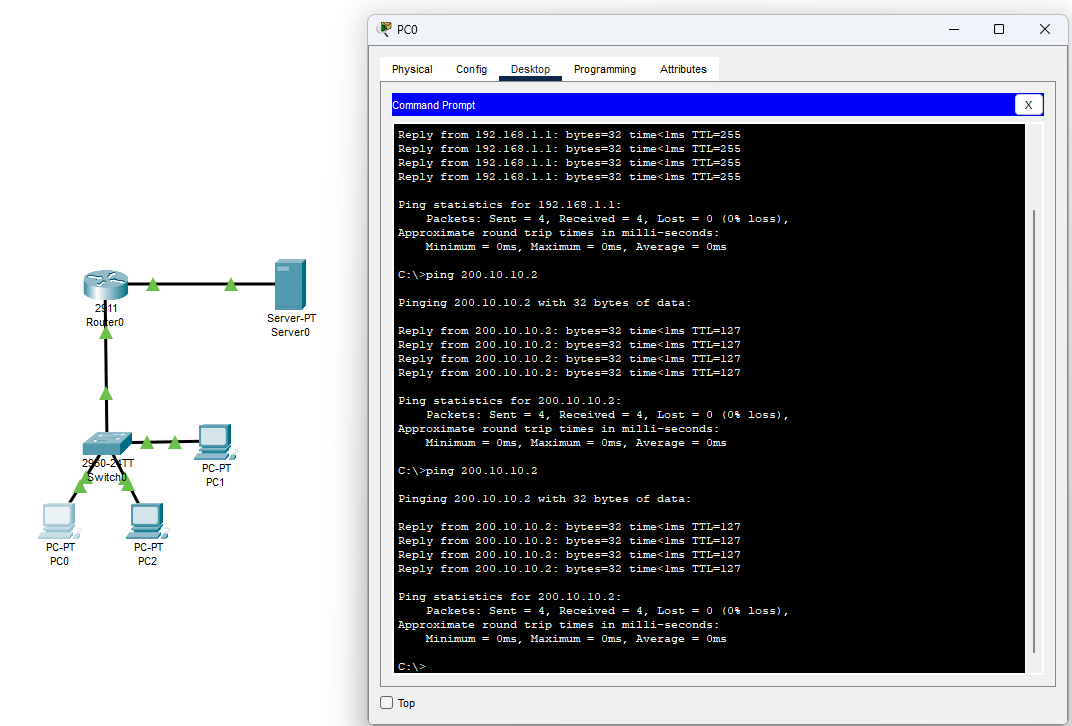
\includegraphics[width=\linewidth]{P1/img/Test Ping ACL Skenario 2 PC0.png}
        \caption{Hasil Ping dari PC0 ke Server (Skenario 2)}
        \label{fig:ping_acl2_pc0}
    \end{minipage}
    \hfill
    \begin{minipage}[t]{0.48\textwidth}
        \centering
        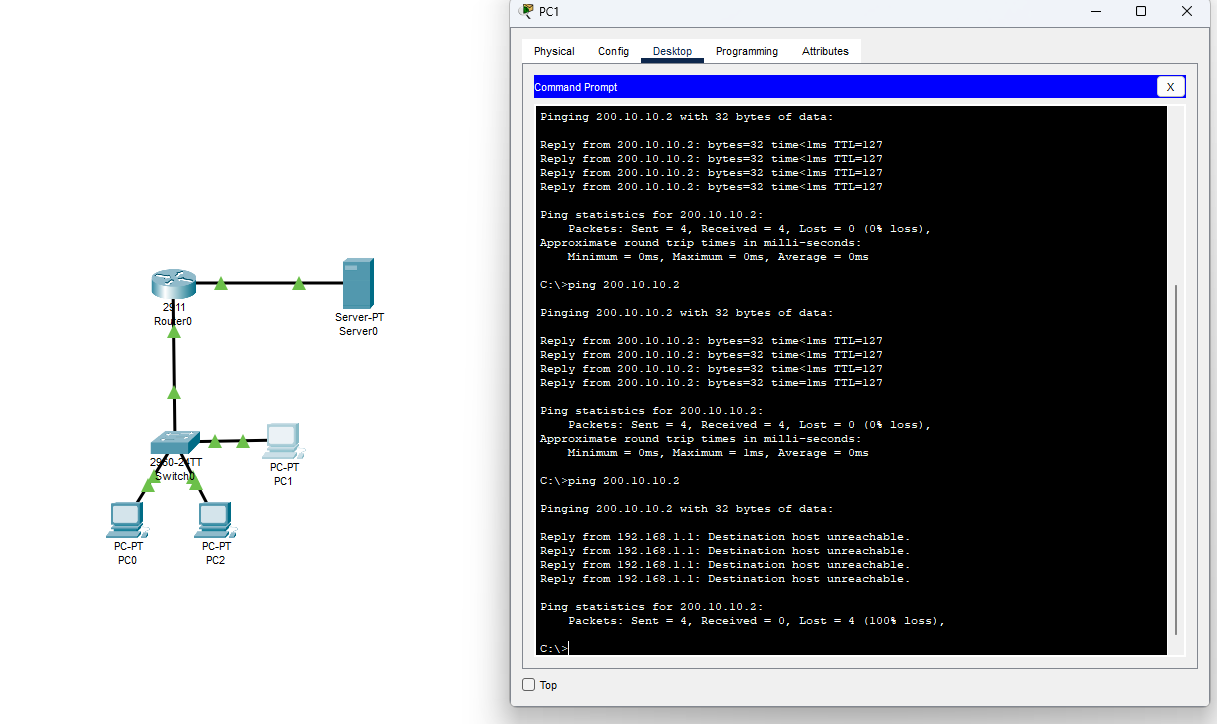
\includegraphics[width=\linewidth]{P1/img/Test Ping ACL Skenario 2 PC1.png}
        \caption{Hasil Ping dari PC1 ke Server (Skenario 2 - Gagal)}
        \label{fig:ping_acl2_pc1}
    \end{minipage}
\end{figure}

\begin{figure}[H]
    \centering
        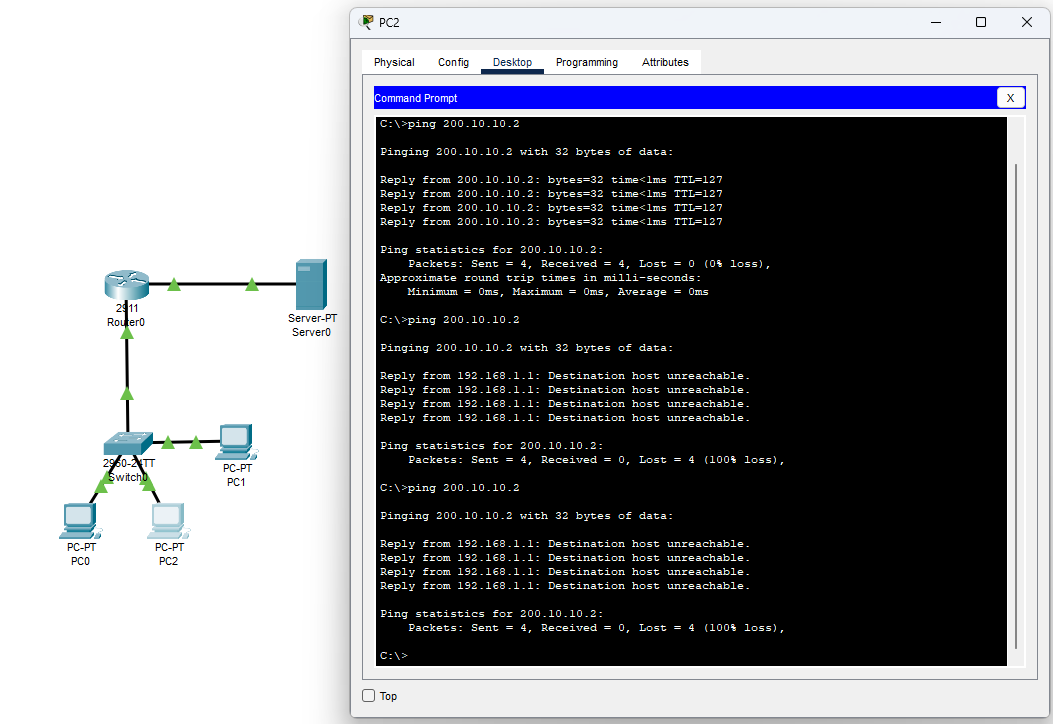
\includegraphics[width=0.48\textwidth]{P1/img/Test Ping ACL Skenario 2 PC2.png}
        \caption{Hasil Ping dari PC2 ke Server (Skenario 2 - Gagal)}
        \label{fig:ping_acl2_pc2}
\end{figure}

\subsection{Kesimpulan Hasil Tugas Modul}
Berdasarkan serangkaian percobaan yang telah dilakukan, semua konfigurasi (topologi dasar, NAT, dan ACL) berhasil diimplementasikan dan diverifikasi di Cisco Packet Tracer. NAT berhasil memungkinkan komunikasi dari jaringan privat ke publik, dan ACLs secara efektif mengontrol akses spesifik antar perangkat, sekaligus mempertahankan konektivitas internal LAN.

\section{Kesimpulan}

Praktikum ini berhasil mengimplementasikan dan memverifikasi fungsionalitas Network Address Translation (NAT) dan Firewall pada perangkat MikroTik RouterBoard. Konfigurasi NAT terbukti efektif dalam menyediakan konektivitas internet bagi perangkat di jaringan lokal. Sementara itu, implementasi Firewall dengan filter rules berhasil memblokir lalu lintas ICMP dan akses ke situs web yang mengandung konten spesifik. Router B juga berhasil dikonfigurasi sebagai bridge, memfasilitasi koneksi perangkat ke jaringan lokal dan perolehan alamat IP dari DHCP Server di Router A. Secara keseluruhan, hasil pengujian menunjukkan bahwa seluruh konfigurasi yang dilakukan bekerja sesuai tujuan, menegaskan pemahaman komprehensif mengenai manajemen jaringan dasar dan keamanan.

\section{Lampiran}

\begin{figure}[H]
    \centering
    \begin{minipage}[t]{0.48\textwidth}
        \centering
        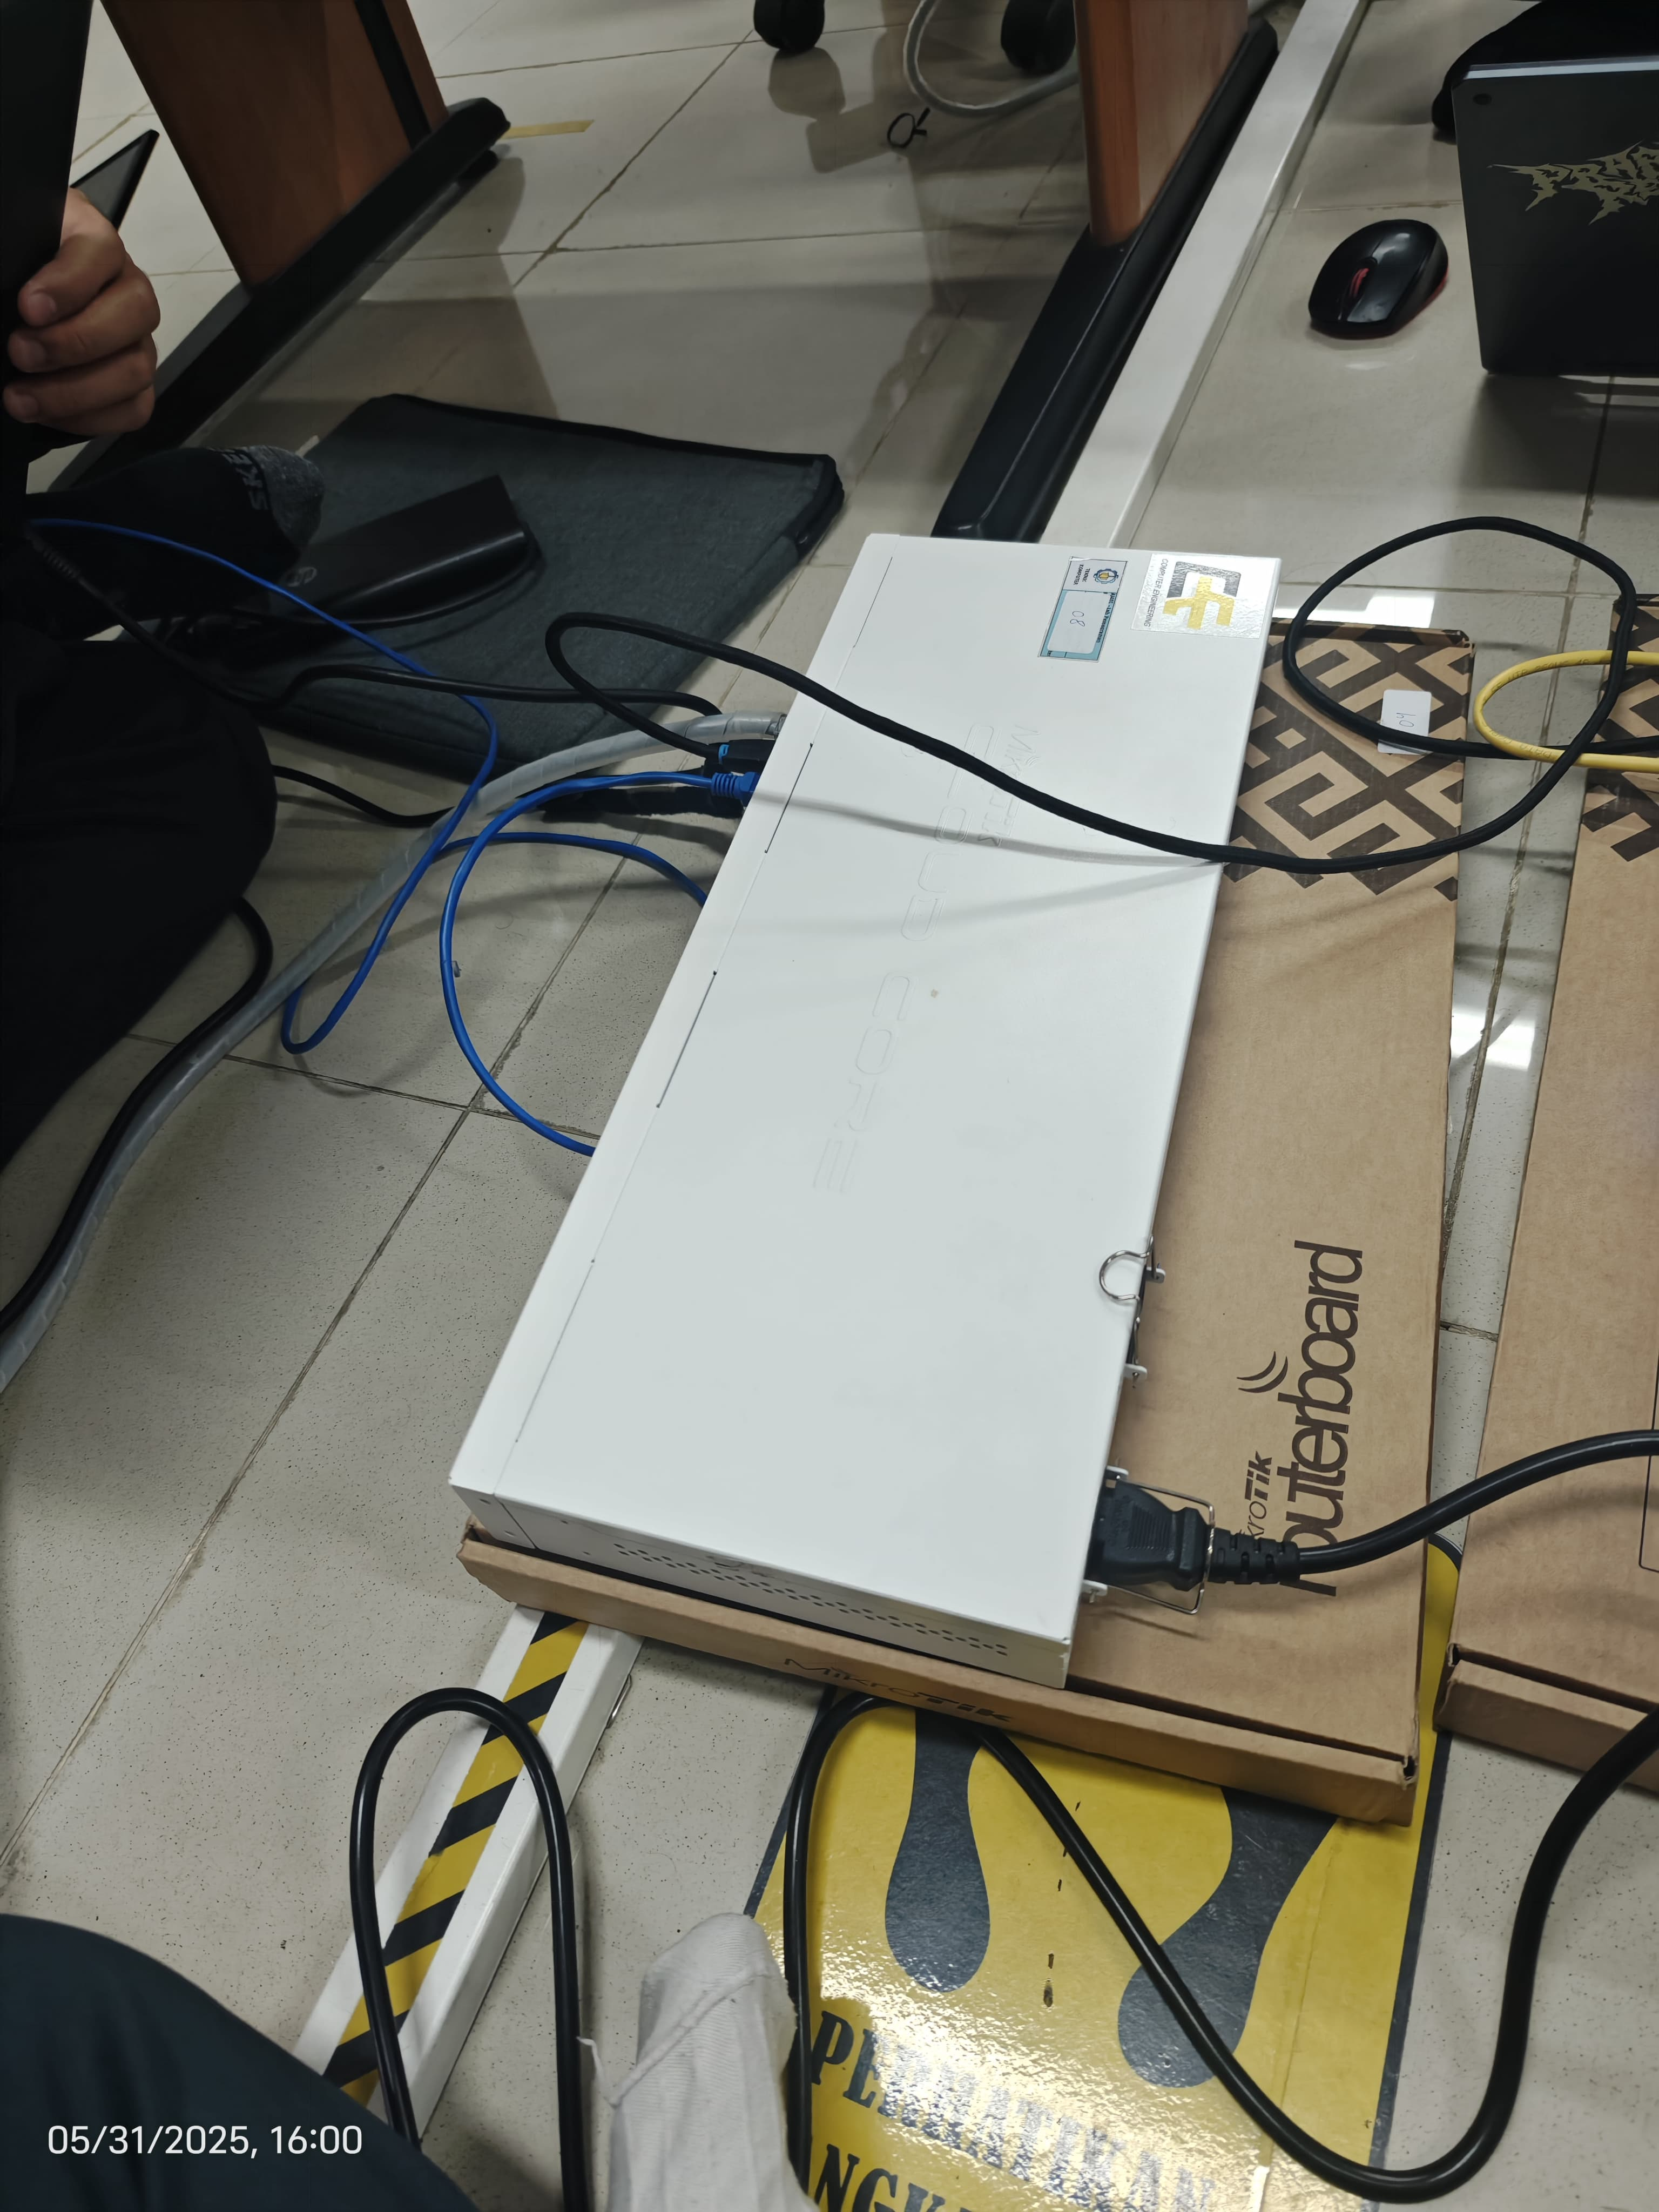
\includegraphics[width=\linewidth]{P1/img/Lampiran5.jpg}
        \caption{Koneksi Kabel pada Router A}
        \label{fig:lampiran5}
    \end{minipage}
    \hfill
    \begin{minipage}[t]{0.48\textwidth}
        \centering
        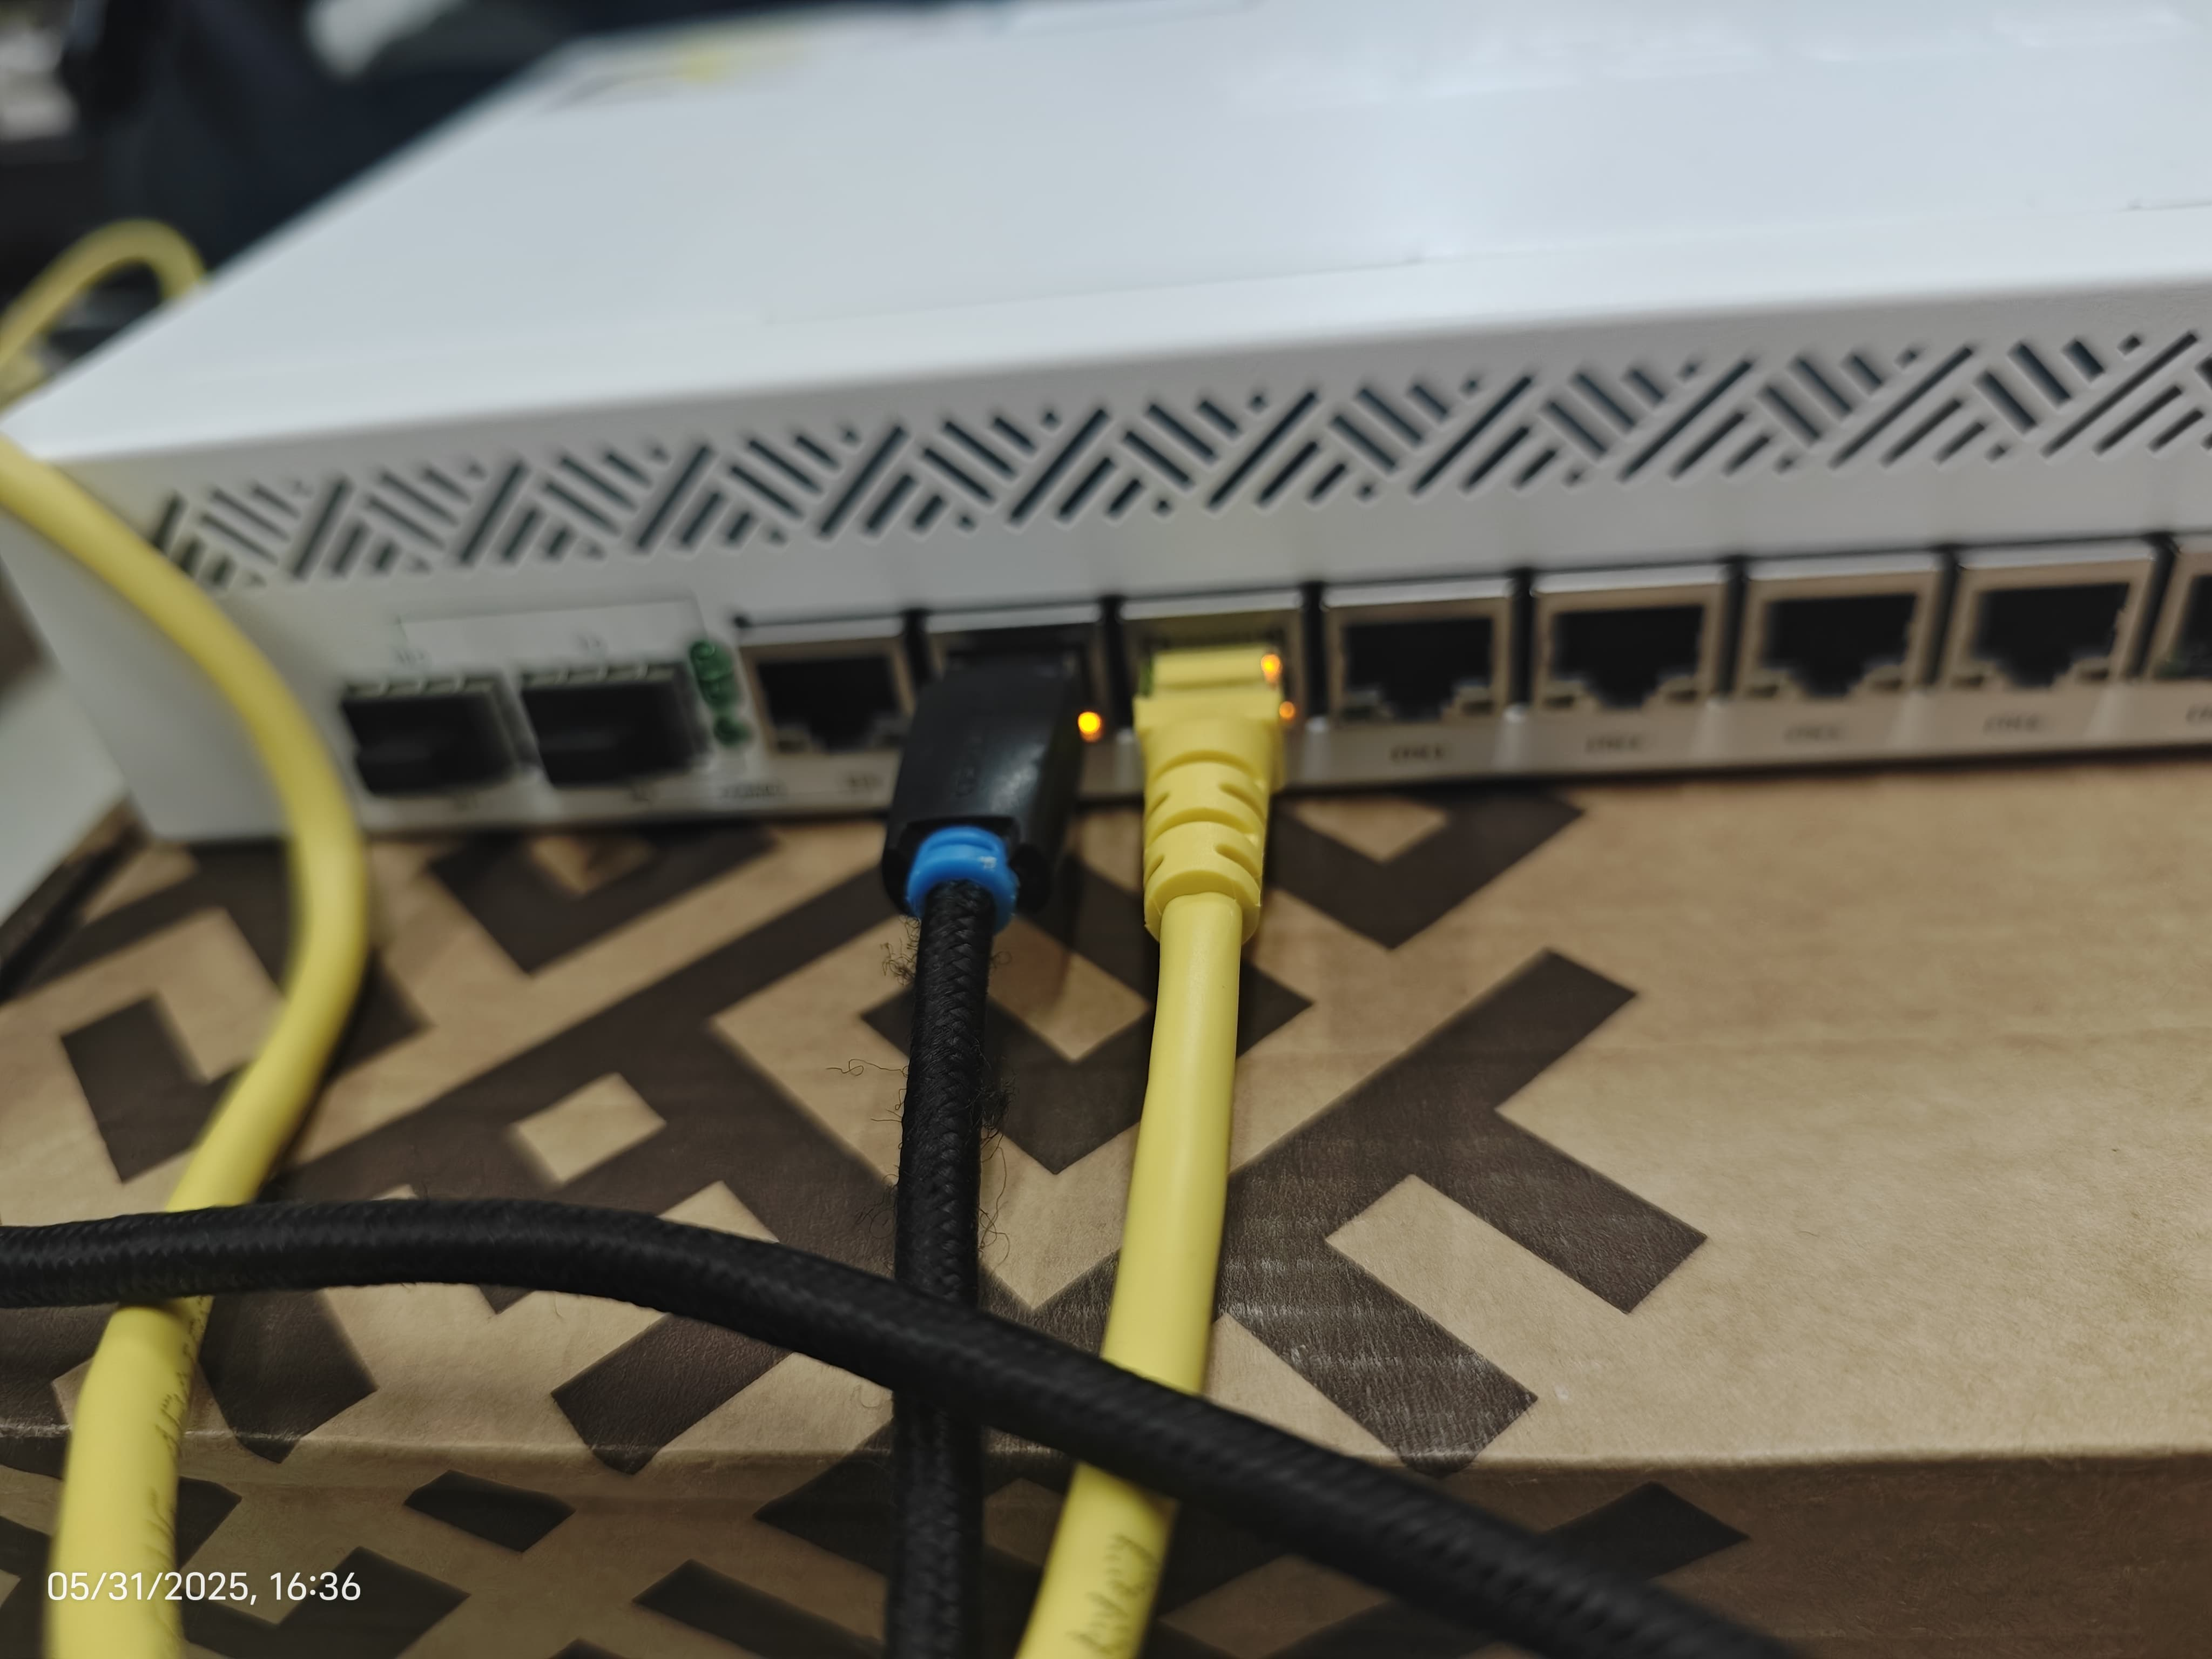
\includegraphics[width=\linewidth]{P1/img/Lampiran6.jpg}
        \caption{Detail Koneksi Kabel Router B}
        \label{fig:lampiran6}
    \end{minipage}
\end{figure}

\begin{figure}[H]
    \centering
    \begin{minipage}[t]{0.48\textwidth}
        \centering
        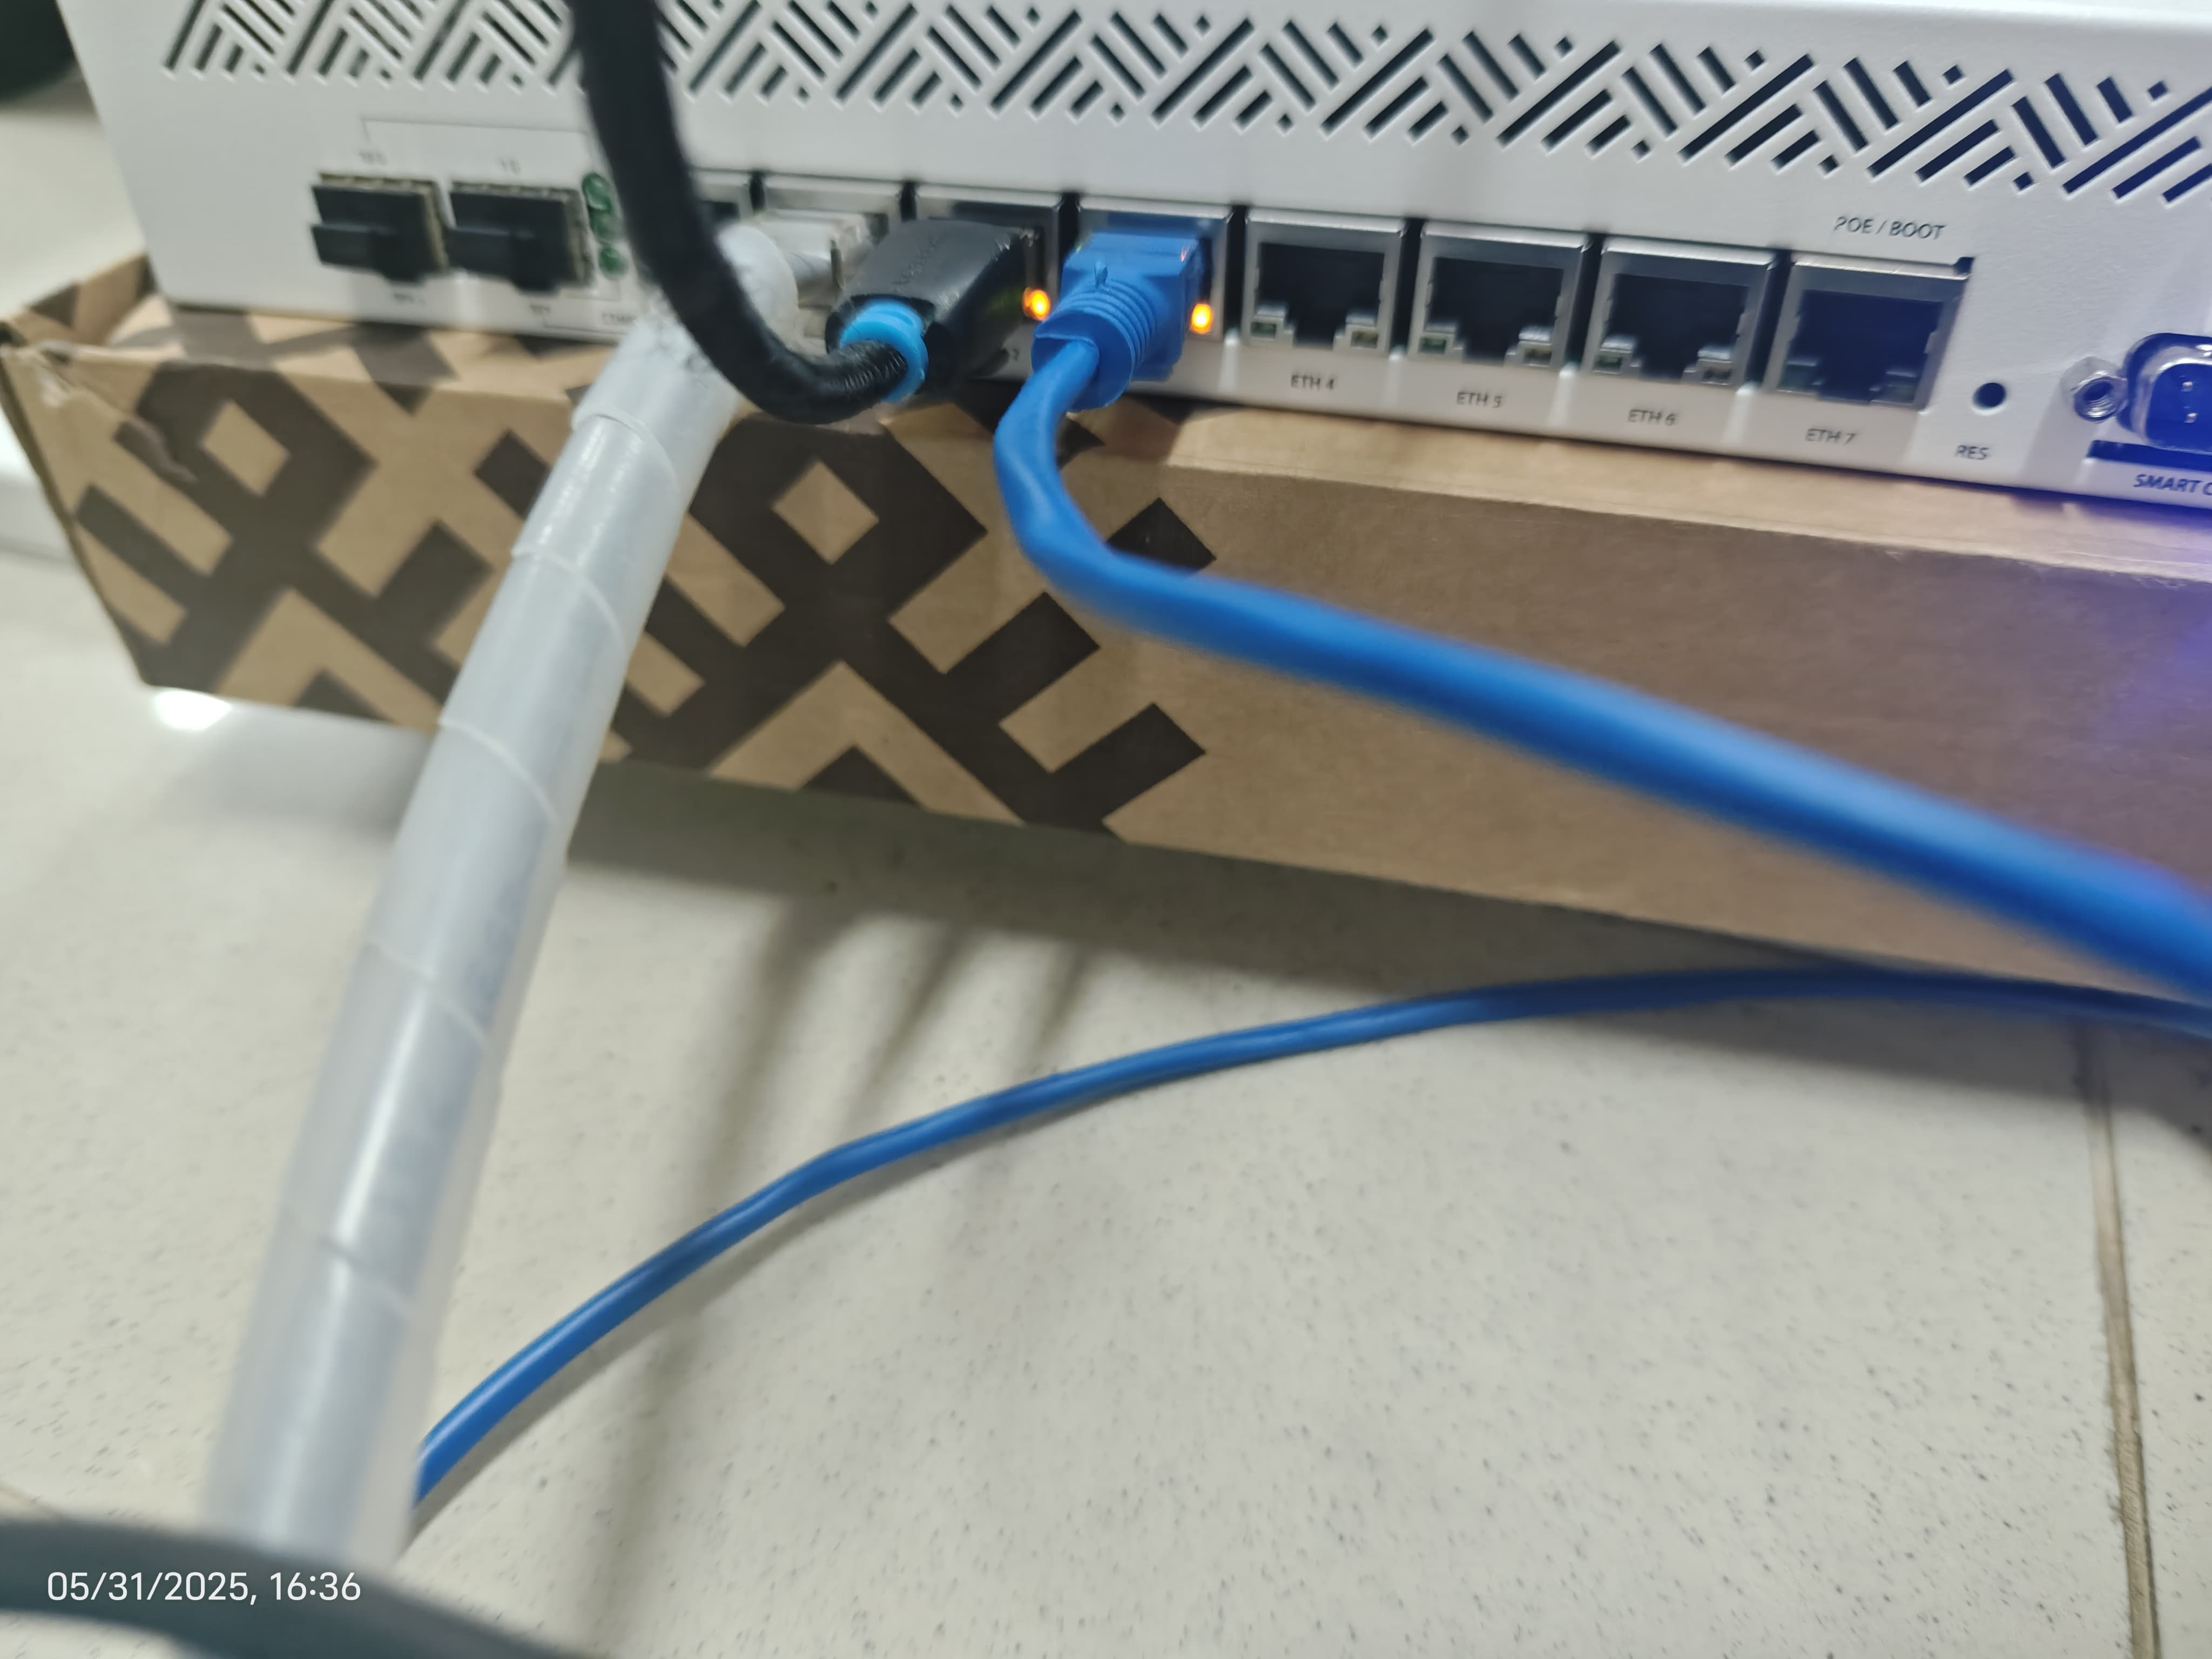
\includegraphics[width=\linewidth]{P1/img/Lampiran7.jpg}
        \caption{Detail Koneksi Kabel Router A}
        \label{fig:lampiran7}
    \end{minipage}
\end{figure}